\chapter{Theoretical aspects}
\pagestyle{fancy}
% \lhead{Theoretical aspects of mining data streams}
\label{relatedWork}
\lstset{style=mystyle}

Most textbooks and computer algorithms on statistical methods will introduce the following ideas: numerical calculations are precise, but graphs are rough; there exists only one set of calculations constituting a correct data analysis; "performing intricate calculations is virtuous, whereas actually looking at the data is cheating". Back in Feb., 1973, F. J. Anscombe was advocating the usefulness of graphs \cite{anscombe}, being essential to good statistical analysis. Scientists often tend to overlook the computations while missing the bigger picture. "There are graphical and analytical means of exploration in data mining, and visualization is one of the most versatile techniques" \cite{hoho}. The proposed approach has an experimental nature, meaning that we have started from a set of assumptions about the behavior of data. Those assumptions may be false, and the calculations may be misleading us, so we will make use of multiple tools, such as graphs, in order to control the truthness of the final results. There will be a red line, holding together this idea that we ought always check if the assumptions made were reasonably correct, and if not, correct them.

Not only the massive data collections, powerful multiprocessor computers and algorithms are solving problems nowadays, but also building cross domain knowledge, especially when paths cannot be found in data that has no meaning for the person who seeks the knowledge. We also took into consideration information extracted from medical journals, blogs and papers relevant to this study.

"Traditional methods, such as statistical process control based on various underlying probability distribution functions, have been successfully implemented in hospital infection control. Data mining techniques have been implemented separately, and some of these are described below. Direct comparison of traditional statistical methods with data mining would require competitive results on the same data. Application of either statistical or data mining techniques requires substantial human effort, and collaboration, rather than competition, needs to occur between the two fields. As more statisticians become involved in data mining, the two fields could contribute to each other more effectively by building on each other's strengths to create synergy than by having a "bake off" or taking an antagonistic approach." [Application of Data Mining Techniques to Healthcare Data Mary K. Obenshain, MAT]

The function with respect to the number of transistors in a dense integrated circuit “can’t continue forever. It is the nature of exponential functions", it will "eventually hit a wall". This corollary was stated by Moore himself, back in 2005. The term “Data Deluge” was coined in 2003 \cite{soton257695} in the context of scientific data management to describe the massive growth in the data volume generated in research (and by scientific instruments), which was rapidly dwarfing all the data previously collected in the history of research. Since then, the ability to generate vast quantities of data has outpaced the infrastructure and support tools.

\begin{figure}[htp]
    \centering
    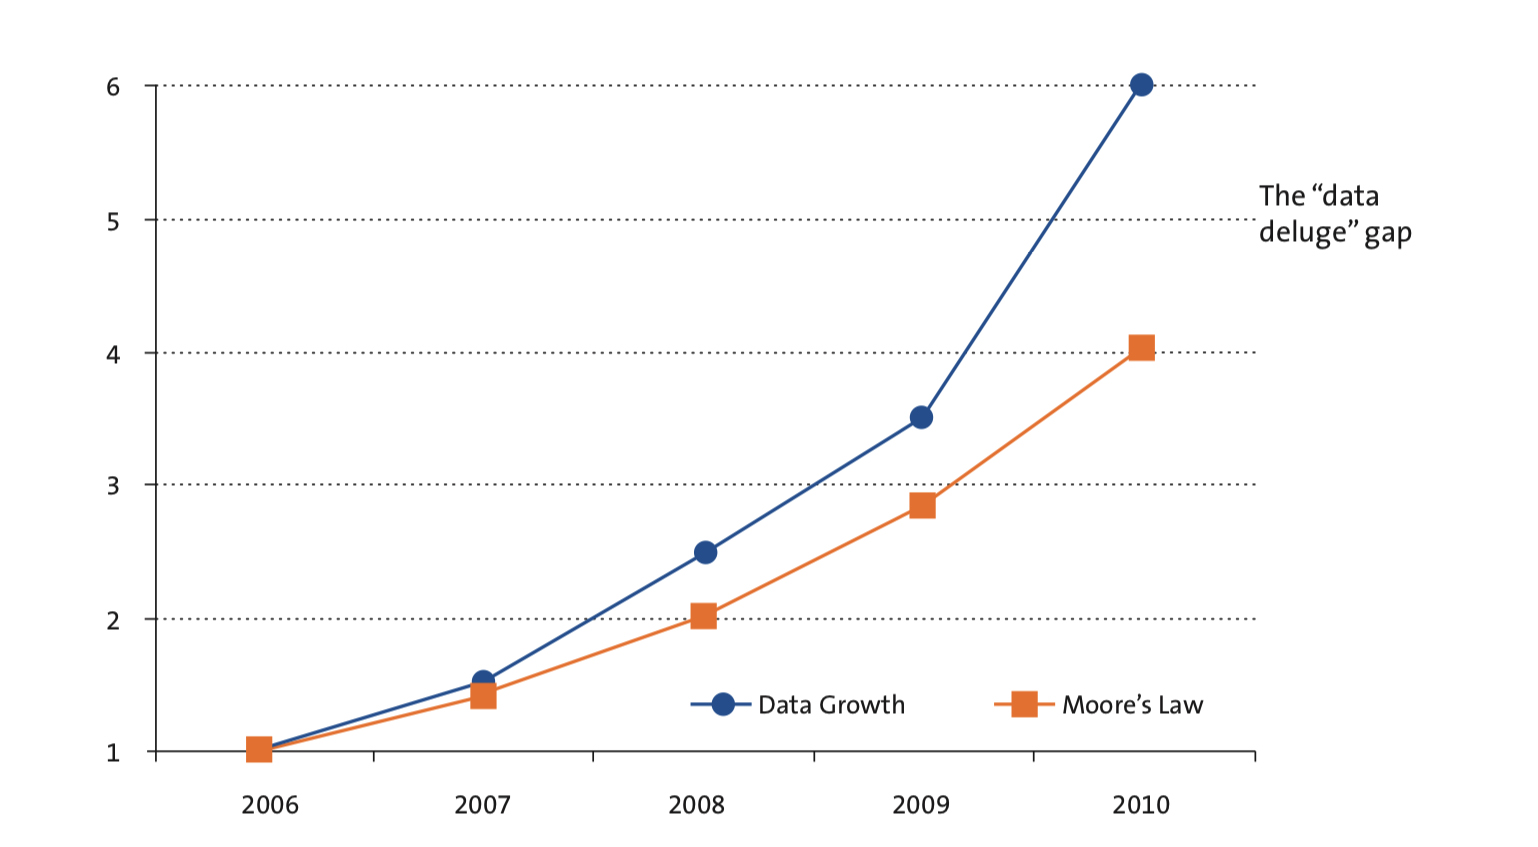
\includegraphics[width = 15.5cm]{figures/MooreVsDataGrowth}
    \caption{Data growth vs. Moore’s Law trends between 2006 and 2010 \cite{HiPEAC}}
    \label{fig:dataDeluge}
\end{figure}

This is true for scientific data, digital media (audio and video), commercial transactions, social networks, legal and medical records, digital libraries, and so on. The need to analyse, organise, and sustain “big data” is one of the highest priorities in information technology across disciplines, organisations and geographies \cite{pvsc}. In 2010 the world generated over 1.2 Zetta bytes (1021 bytes) of new data, 50\% more than everything produced in human history before that year. To put this in perspective, 120 Terabytes of new data was generated in the time it took to read the previous sentence. In short, data “deluge” means that we are heading towards a world where we will have more data available than we can process. \cite{HiPEAC}

If there is one thing that we must take into account next time we develop an application, is how to build it, so that we prevent it from falling under the huge amounts of data we collect. The application described in this paper is designed to overcome those shortcomings through the event ingestion layer and the event source points that can be redesigned. Part of the data we collect becomes obsolete over the time and can be discarded, but we must design our tables with a certain degree of freedom, so that data deletion won't be prevented.

\section{Data mining}

Traditional machine learning algorithms were designed to discover knowledge and experience by themselves in a limited data set, yet the problem changes when data sets become larger, the structures more complicated and data is not always following the same schema. Sometimes, in competitive programming, we can find ourselves searching for clues in data sets of around $10^3$ tuples. Small details can make the difference in a competition - knowing if the elements are repeating themselves, which are the boundaries for a field or how is the last improvement affecting the final score. Even small patterns can make a great difference. Therefore, data mining is a method of finding paths hidden in plain sight.

\begin{figure}[ht!]
    \centering
    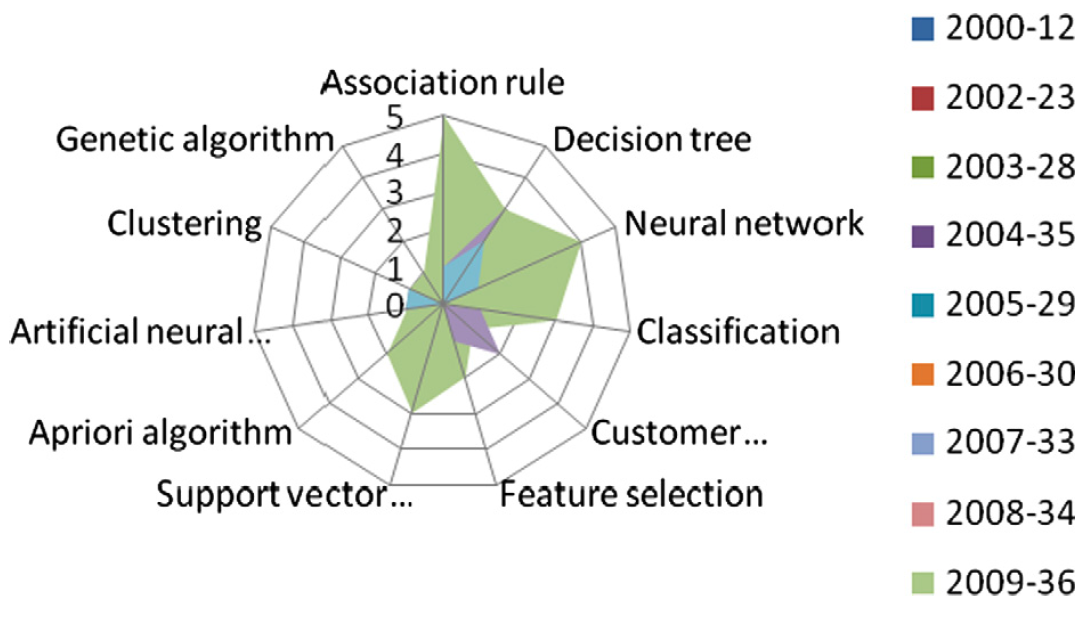
\includegraphics[width = 15.5cm]{figures/dmt}
    \caption{Data mining trend from 2000-2011 \cite{LIAO201211303}}
    \label{fig:dmt}
\end{figure}

\subsubsection{Strategies}

"Supervised learning methods are deployed (or strategically put into service in an information technology context) when values of variables (inputs) are used to make predictions about another variable (target) with known values. Unsupervised learning methods can be used in similar situations, but are more frequently deployed on data for which a target with known values does not exist. An example of a supervised method would be a healthcare organization finding out through predictive modeling what attributes distinguish fraudulent claims. In supervised methods, the models and attributes are known and are applied to the data to predict and discover information. With unsupervised modeling, the attributes and models of fraud are not known, but the patterns and clusters of data uncovered by data mining can lead to new discoveries." \cite{hoho}

\begin{table}[ht!]
  \begin{center}
    \label{tab:table9}
    {\begin{tabular}{l|l|l}
      \textbf{Modeling Objective} & \textbf{Supervised} & \textbf{Unsupervised}\\
      \hline
       Prediction & Ordinary least squares regression & Not feasible \\
       & Logistic regression &\\
       & Neural networks &\\
       & Decision trees &\\
       & Memory-based reasoning &\\
       & Support vector machines &\\
       & Multi-adaptive regression splines &\\
       Classification & Decision trees & Clustering (K means) \\
        & Neural networks & Kohonen networks \\
        & Discriminant analysis & Self-organizing \\
        & Bagging and boosting ensembles & \\
        & Naive Bayes classifiers & \\
       Exploration & Decision trees & Principal components \\
       & & Clustering (K means) \\
       & & Link analysis \\
    \end{tabular}}
  \end{center}
\end{table}

"Prediction algorithms determine models or rules to predict continuous or discrete target values given input data. For example, a prediction problem could involve attempting to predict the amount of an insurance claim or a death rate given a set of inputs (pick one and then list the corresponding inputs). Classification algorithms determine models to predict discrete values given input data. A classification problem might involve trying to determine whether a particular purchase represents anomalous behavior based on some indicators (eg, where the purchase was made, the amount of the purchase, or the type of purchase). Exploration uncovers dimensionality in input data. Trying to identify groups of similar customers based on spending habits for a large, targeted mailing is an exploration problem. Affinity analysis determines which events are likely to occur in conjunction with one another. Retailers use affinity analysis to analyze product purchase combinations in grocery stores." \cite{hoho}

\subsubsection{Similar approach for data mining bike sharing demand prediction in metropolitan city}

In \cite{E2020353}, the authors are discussing a couple of models for hourly rental bike demand prediction. An interesting aspect of this paper is that it uses similar weather measurements (Temperature, Humidity, Windspeed, Visibility, Dewpoint, Solar radiation, Snowfall, Rainfall), the number of bikes rented per hour and date information. The paper also explores "a filtering of features approach to eliminate the parameters which are not predictive and ranks the features based on its prediction performance. Five Statistical regression models were trained with their best hyperparameters using repeated cross-validation and the performance is evaluated using a testing set: (a) Linear Regression (b) Gradient Boosting Machine (c) Support Vector Machine (Radial Basis Function Kernel) (d) Boosted Trees, and (e) Extreme Gradient Boosting Trees. When all the predictors are employed, the best model Gradient Boosting Machine can give the best and highest R2 value of 0.96 in the training set and 0.92 in the test set" \cite{E2020353}.

\subsubsection{Understanding pattern's discovery in drug trials using SEMMA}

Research made in the area of drugs discovery can be accelerated with real time data exploration as the throughput of candidates for clinical trials have significantly increased in the last couple of years, and the time required for drugs preparation decreased. Using streaming tools also alleviate the burden of high throughput. "Twenty years ago, pharmaceutical scientists could screen approximately 30 drug candidates per week. Today, with combinatorial chemistry and high throughput screening, the same scientists can screen thousands of compounds per day in a controlled biological assay to determine potentially effective treatments. The most effective compounds, called “hits,” are classified and retested. The best “leads” may result in a chemical synthesis program to optimize the chemical structure regarding the biological activity of interest" \cite{hoho}. A scientist can study the relationship between chemical structures and biological activity in a real-time manner. After patterns were discovered, the next step is finding the cause of those patterns. "Numerous modeling techniques are available, including traditional statistics. Some market analysts may include visualization as a modeling technique, but the SEMMA method finds an earlier place for this in the exploration phase" \cite{hoho}. It stands for Sample, Explore, Modify, Model, and Assess, a list of sequential steps used for guiding the implementation of data mining applications.


\begin{table}[ht!]
  \begin{center}
    \label{tab:table5}
    {\begin{tabular}{p{2cm} p{12cm}}
        \textbf{Step} & \textbf{Description} \vspace{2mm} \\
        \hline
         Sample & Mining a representative sample of the initial population decreases the processing time required to begin the knowledge exploration. Estimating population parameters given a representative sample is a well established topic in statistics. If patterns appear in the data as a whole, these will be traceable in a representative sample as well. In \cite{hoho} the goal is to relate chemical structure to biological activity. Because nobody can know how well the results are going to be generalized to other data sets, a common way is to create partitions of the given data set. Partitions can be generated as data comes into the system. \vspace{2mm} \\
         Explore & Visualization is one of the most versatile techniques when exploring large data sets. In the drug discovery examples described above, scientists graphically examined different variables. Even though it was not described in the theoretical section, Google Cloud also provides tools for graphically summarization. \vspace{2mm}\\
         Modify & Data quality is essential in this problem and it might have records with missing values or outliers that could obstruct some of the patterns. Removing those records can be a solution, but instead of removing data we can replace them with a mean, a median, or user-specified method.\vspace{2mm} \\
         Model & Because not all methods are suitable for all data, we should choose those that harness knowledge without bending the problem in order to fit a particular method. \vspace{2mm}\\
         Assess & In the preliminary stages of the study neural networks seemed to be the best model, having better results than the logistic regression and the decision tree, capturing more of the best compounds more quickly. Even so, a later examination of scores revealed that the neural network did better than the logistic regression but not as well as the decision tree in identifying active compounds. "Thus, in the process flow diagram, the output model was changed from neural networks to decision tree so that the tree-based model will be used for subsequent predictions." \cite{hoho} \\
         
    \end{tabular}}
  \end{center}
\end{table}

\clearpage
\section{Data streams}

A data stream is a countably infinite sequence of elements and is used to represent data elements that are made available over time. Data stream management systems are designed to update the answers of continuous queries as new data becomes available. They typically adopt declarative abstractions similar to traditional database query languages that they enrich with constructs such as windows to deal with the unbounded nature of the input data. \cite{defs}

Streaming systems have been associated with low-latency, inaccurate, or speculative results, whereas more capable batch systems provided the correct results. The "broad maturation of streaming systems combined with robust frameworks for unbounded data processing will in time allow for the relegation of the Lambda Architecture to the antiquity of big data history where it belongs”, said Tyler Akidau in the book called Streaming Systems. Lambda architecture is an attempt to balance latency, throughput, and fault-tolerance by using batch processing for a correct data analysis, while streaming for a real-time overview. Lambda Architecture systems fail on the simplicity, having to build and maintain two systems \cite{TheDataflowModel}. We can humbly add that the existing DSMS \footnote{Data Stream Management System} are not mature enough, yet they will be soon enough.

The first interaction with a streaming system produced me the mental image of an additional layer over a classic DBMS \footnote{Database Management System}, handling the massive throughput of incoming data. This perception led to the Greek mythological figure known under the name of Atlas. The titan was punished to bear the weight of the heavens on his shoulders, for his actions in the battle against the gods.

For the current application, the ingestion rates of a streaming system can be associated with the following magnitudes:
\begin{table}[h!]
  \begin{center}
    \label{tab:table1}
    \caption{Ingestion magnitude}
    \begin{tabular}{l|r} % <-- Alignments: 1st column left, 2nd middle and 3rd right, with vertical lines in between
      \textbf{large throughput} & \textbf{narrow throughput}\\
      generated by sensors & produced by outdoor activities\\
      \hline
      light & running\\
      temperature & cycling\\
      air pressure & \\
    \end{tabular}
  \end{center}
\end{table}

Streaming data, even at low rates, enables us with the proper tools to react with small, unnoticeable delays. Because of the ingestion abilities of its kind, streaming engines permit a couple of business processes to go real-time. The most recent stage in the development of hardware and software capabilities allows a model to be continuously updated in an upper-bounded time interval instead of manually triggering or planning in advance the following update. An interesting comparison arises on the streaming vs batch systems in terms of performance. Computation can be distributed over time as activities are performed, unlike buffering those until a threshold is reached. Spanning 10 activities from 10k people over a week can reduce the stress the system experiences, as the schedule world-wide permits to consider activities having place 24 hours out of 24. This idea is supported by a paragraph from \cite{ACL}, saying that processing "data as they arrive spreads workloads out more evenly over time, yielding more consistent and predictable consumption of resources".

As an example, in Figure \ref{fig:strava} is presented a graph Carlin Eng pulled back in 2014, showing Strava \footnote{Strava is a free digital service focused on fitness tracking} usage by day of the week (published at labs.strava.com). The orange line tracks the count of uploading active members by day, while the blue line tracks non-uploading active members (e.g., someone who has not uploaded an activity, but still logs into Strava to view/comment/kudo an activity).

\begin{figure}[htp]
    \centering
    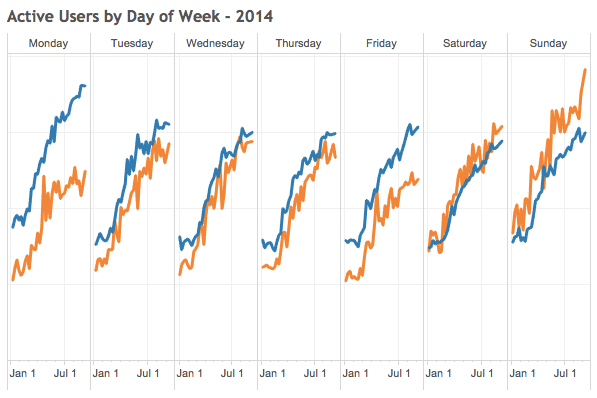
\includegraphics[width = 14cm]{figures/strava}
    \caption{Active users by day of week - 2014}
    \label{fig:strava}
\end{figure}

\section{Cloud computing}

Although the Internet of Things (IoT) has been around for nearly twenty years, it became a reality at large scale only during the past couple of years. In a recently published paper called "Evaluation of IoT stream processing at edge computing layer for semantic data enrichment" the authors propose the idea that this paradigm shift in IoT computing "is due to many factors such as the continuous \textbf{improvements in networking}, processing and data storage \textbf{capabilities of Cloud computing}, which is the real factor for giving IoT such a prevalent role" \cite{xhafa_evaluation_2020}. Combined with the "unlimited capacity in processing power and data storage of Cloud data centers, it is possible not only to extract useful information from IoT data but most importantly to build knowledge, intelligence and decision making systems. Popular names in the technology industry are already taking advantage of the context of smart interconnected devices. For instance, in IBM IoT Cloud, data collected from Arduino or Raspberry Pis is transmitted to IBM Cloud Node-Red servers. Then, the IBM Watson Analytics service processes the IoT data to generate knowledge and intelligence, which can finally be integrated into business workflows of enterprises". \cite{xhafa_evaluation_2020}

\subsection{Internet of Things}

The Internet of Things sounds pretty generic if you are unfamiliarized with this term, but we are surrounded by this technology everyday. To introduce the broad concept of physical devices connected over the internet it is necessary to talk about IoT first. In the broadest sense, the term IoT groups together everything connected to the internet, but it is increasingly being used to define objects that are sharing data between them, like in a conversation. The physical world is the place where technological development encountered some difficulties and stopped. So, by creating a network of physical devices capable of exchanging data between them, it is possible to "gather information, analyse it and create an action" to help someone with a particular task, or learn from a process. \cite{WiredIoT} An interesting exemplification of a use case for physical devices sharing knowledge, that usual people can relate to can be the following: if you bracelet detects that you are running it can check the fridge stock of milk and the wardrobe for dry clothes, so that it notifies you to stop by and shop for some milk, or wash some new running clothes for tomorrow. 

\begin{figure}[!htb]
    \centering
    \begin{tabular}{cc}
        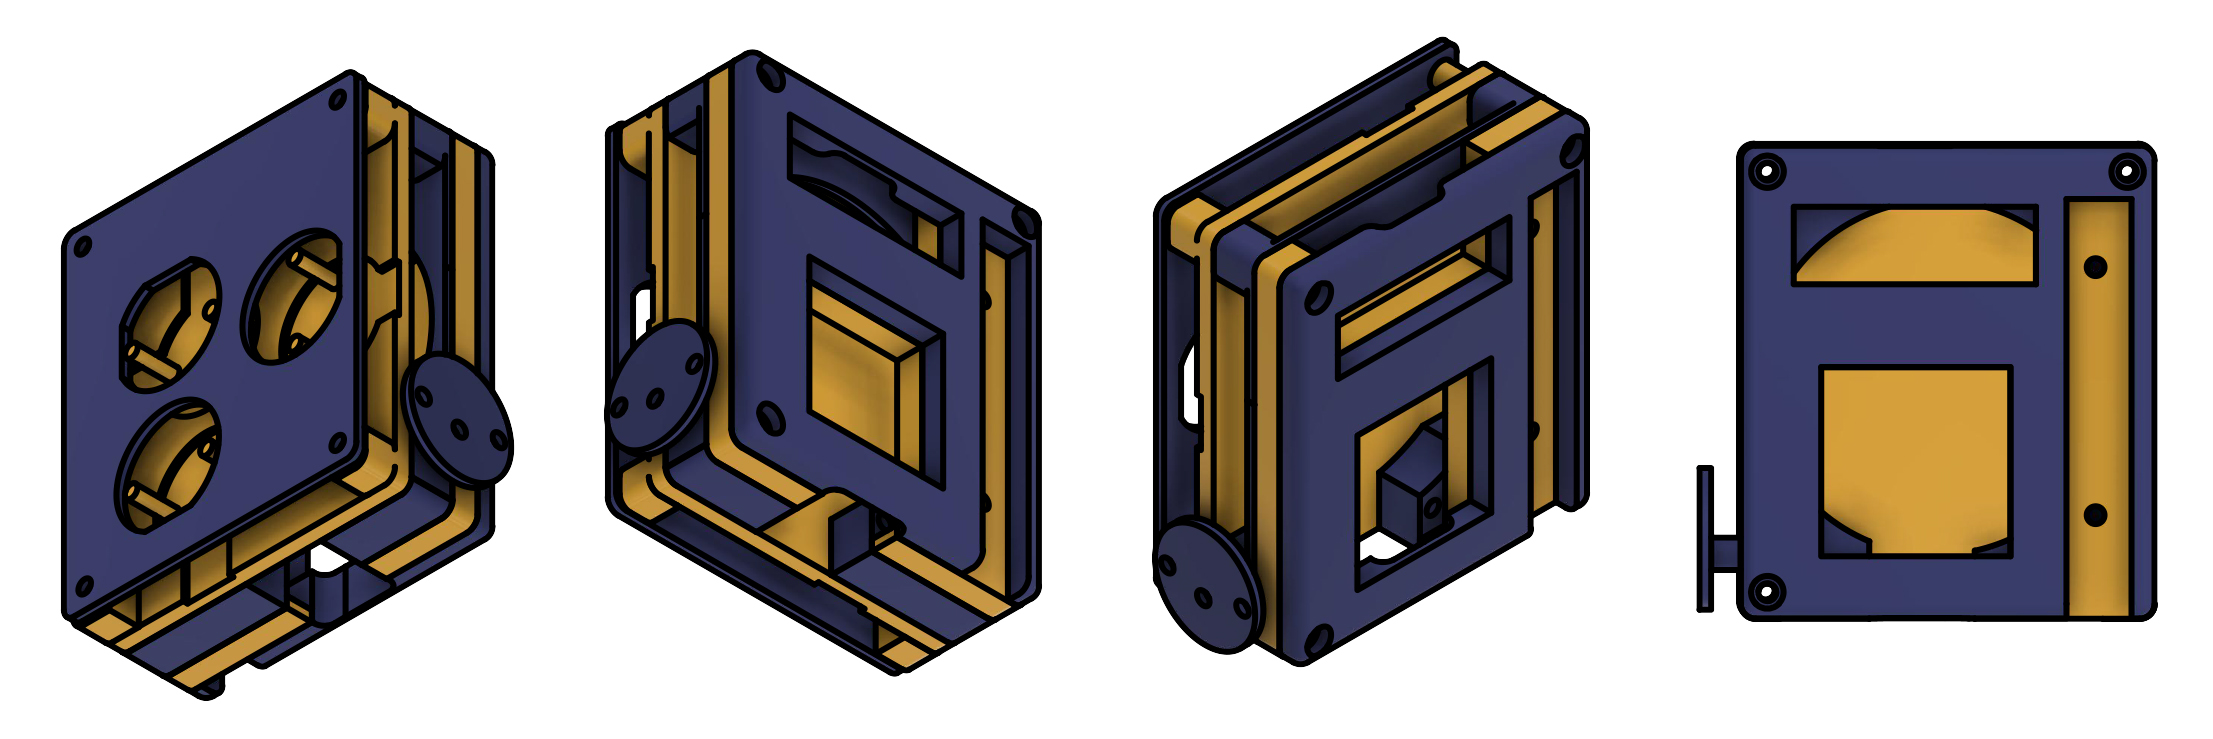
\includegraphics[width=15.5cm]{figures/final-pro-narrow}
    \end{tabular}
    \caption{Drawing schematics for the weather monitor station}
    \label{fig:schematics}
\end{figure}

IoT is a rapidly evolving research topic. According to Scopus, the phrase “Internet of Things” was coined in 1991, but overall search activity on the term did not show significant growth until 2010. We could add that even if this growth was seen in 2010, it took a couple of extra years to see any real world development taking place. (rewrite this with current data) A current search on Scopus for IoT returns a total of 57270 documents when filtered for the past 10 years (2010–2020). The growth in the number of documents related to IoT during this time period reflects the swift emergence of IoT as a research focus in academia, industry and government, as well as the steadily increasing importance of the topic in the overall economy. Conference papers are the largest source for research related to IoT. This accounts for about 58\% of all documents, followed by articles (32\%) and all other sources (10\%), according to a Scopus report we exported on 16 Apr 2020.

\subsection{Rapid prototyping}

For a complete, but very ugly formatted title, this section would be called "Rapid prototyping using open source electronics and 3D printed models". The 3D printing process has deep implications in manufacturing, medical, industry and sociocultural sectors because it allows a wide variety of experts to solve open questions by rapid prototyping. Rapid prototyping is a group of techniques used to quickly fabricate a scale model of a physical part or assembly using three-dimensional computer aided design data. The 3D printing process builds a three-dimensional object from a CAD model, usually by successively adding material layer by layer. In the 1990s, 3D printing techniques were considered suitable only for the production of functional or aesthetic prototypes hence the term of rapid prototyping. As of 2020, the precision, repeatability, and material range have increased to the point that some 3D-printing processes are considered viable as an industrial-production technology. In Figure \ref{fig:printingTheModel} one can observe the printing process of the weather station used in this project.

\begin{figure}[!htb]
    \centering
    \begin{tabular}{lll}
        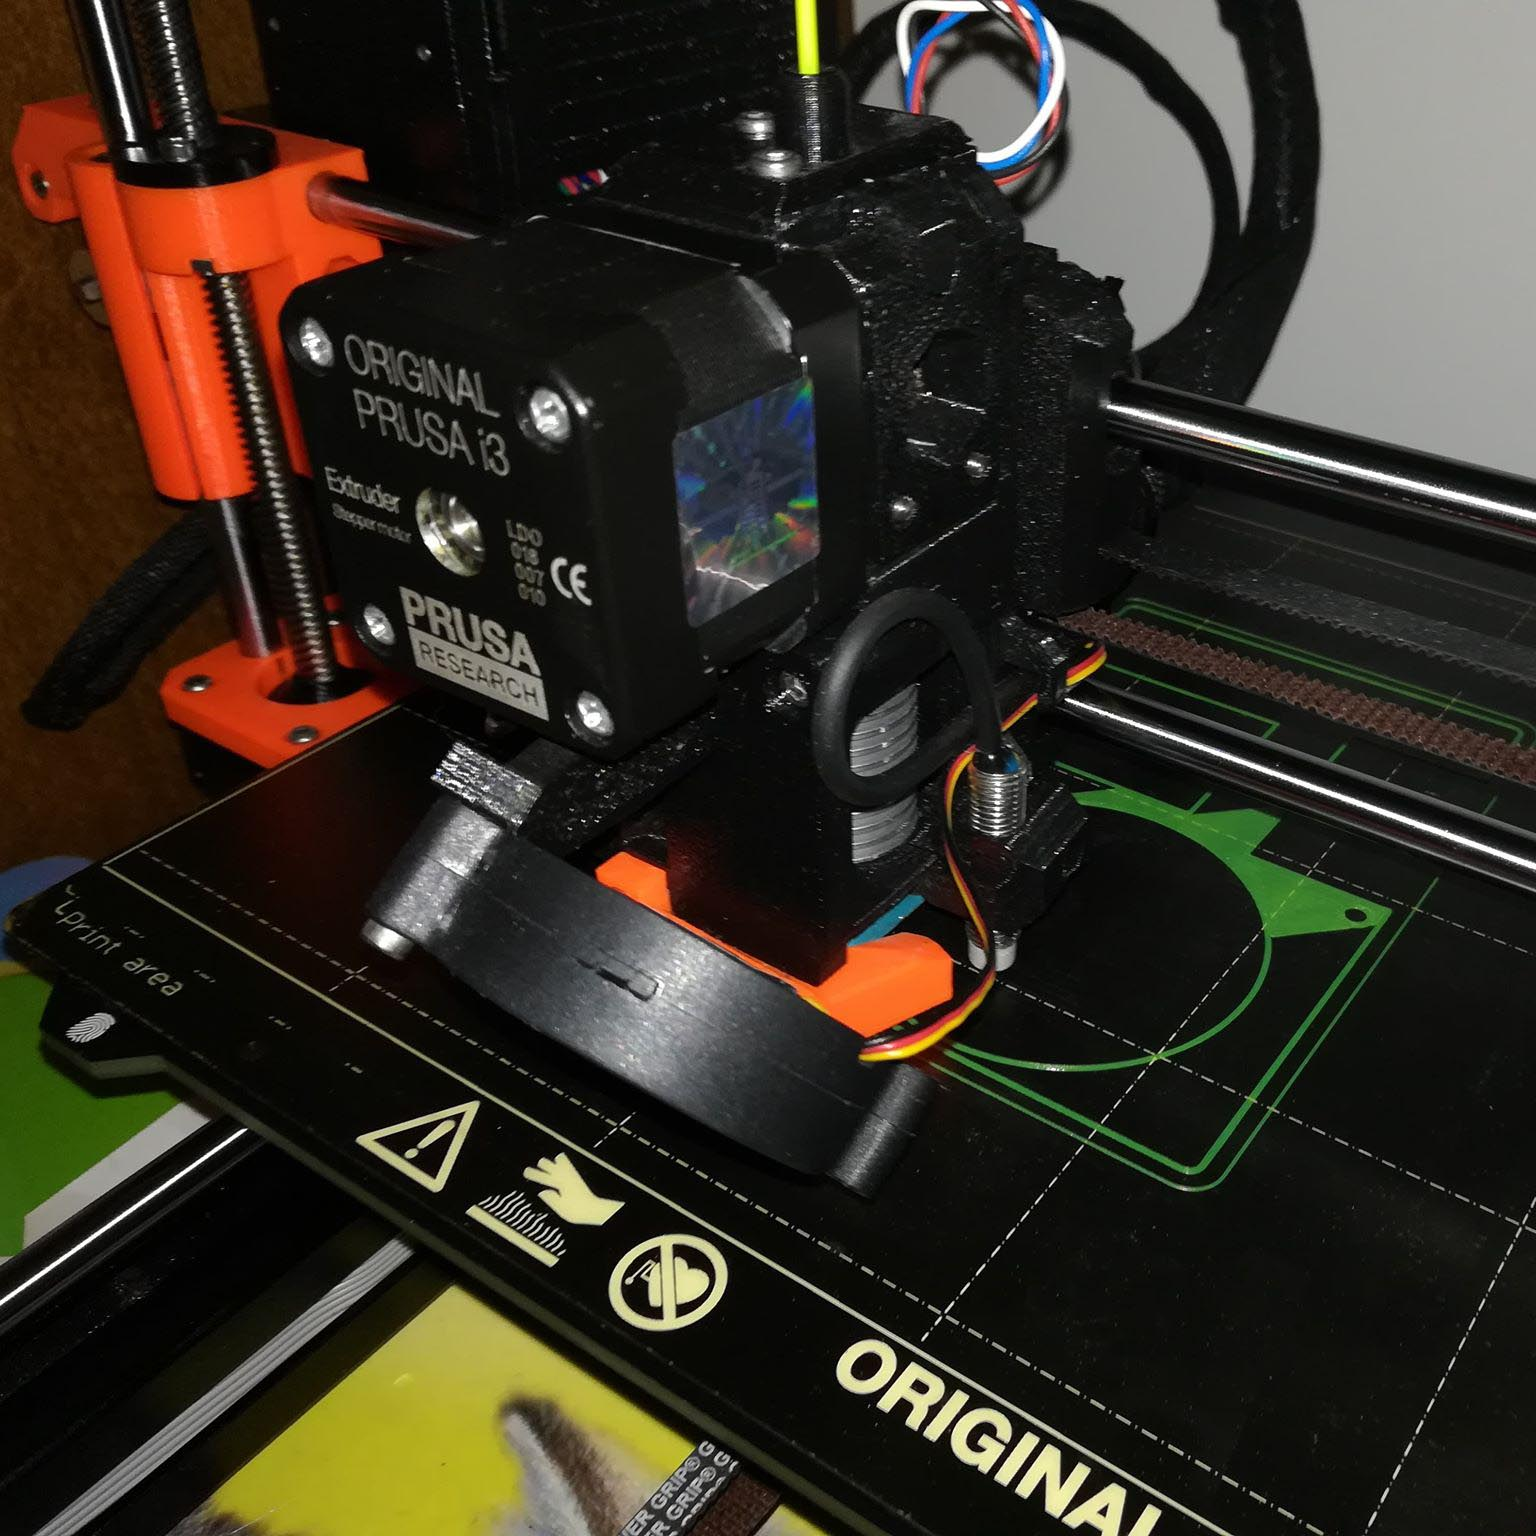
\includegraphics[width=4.8cm]{figures/print2} &
        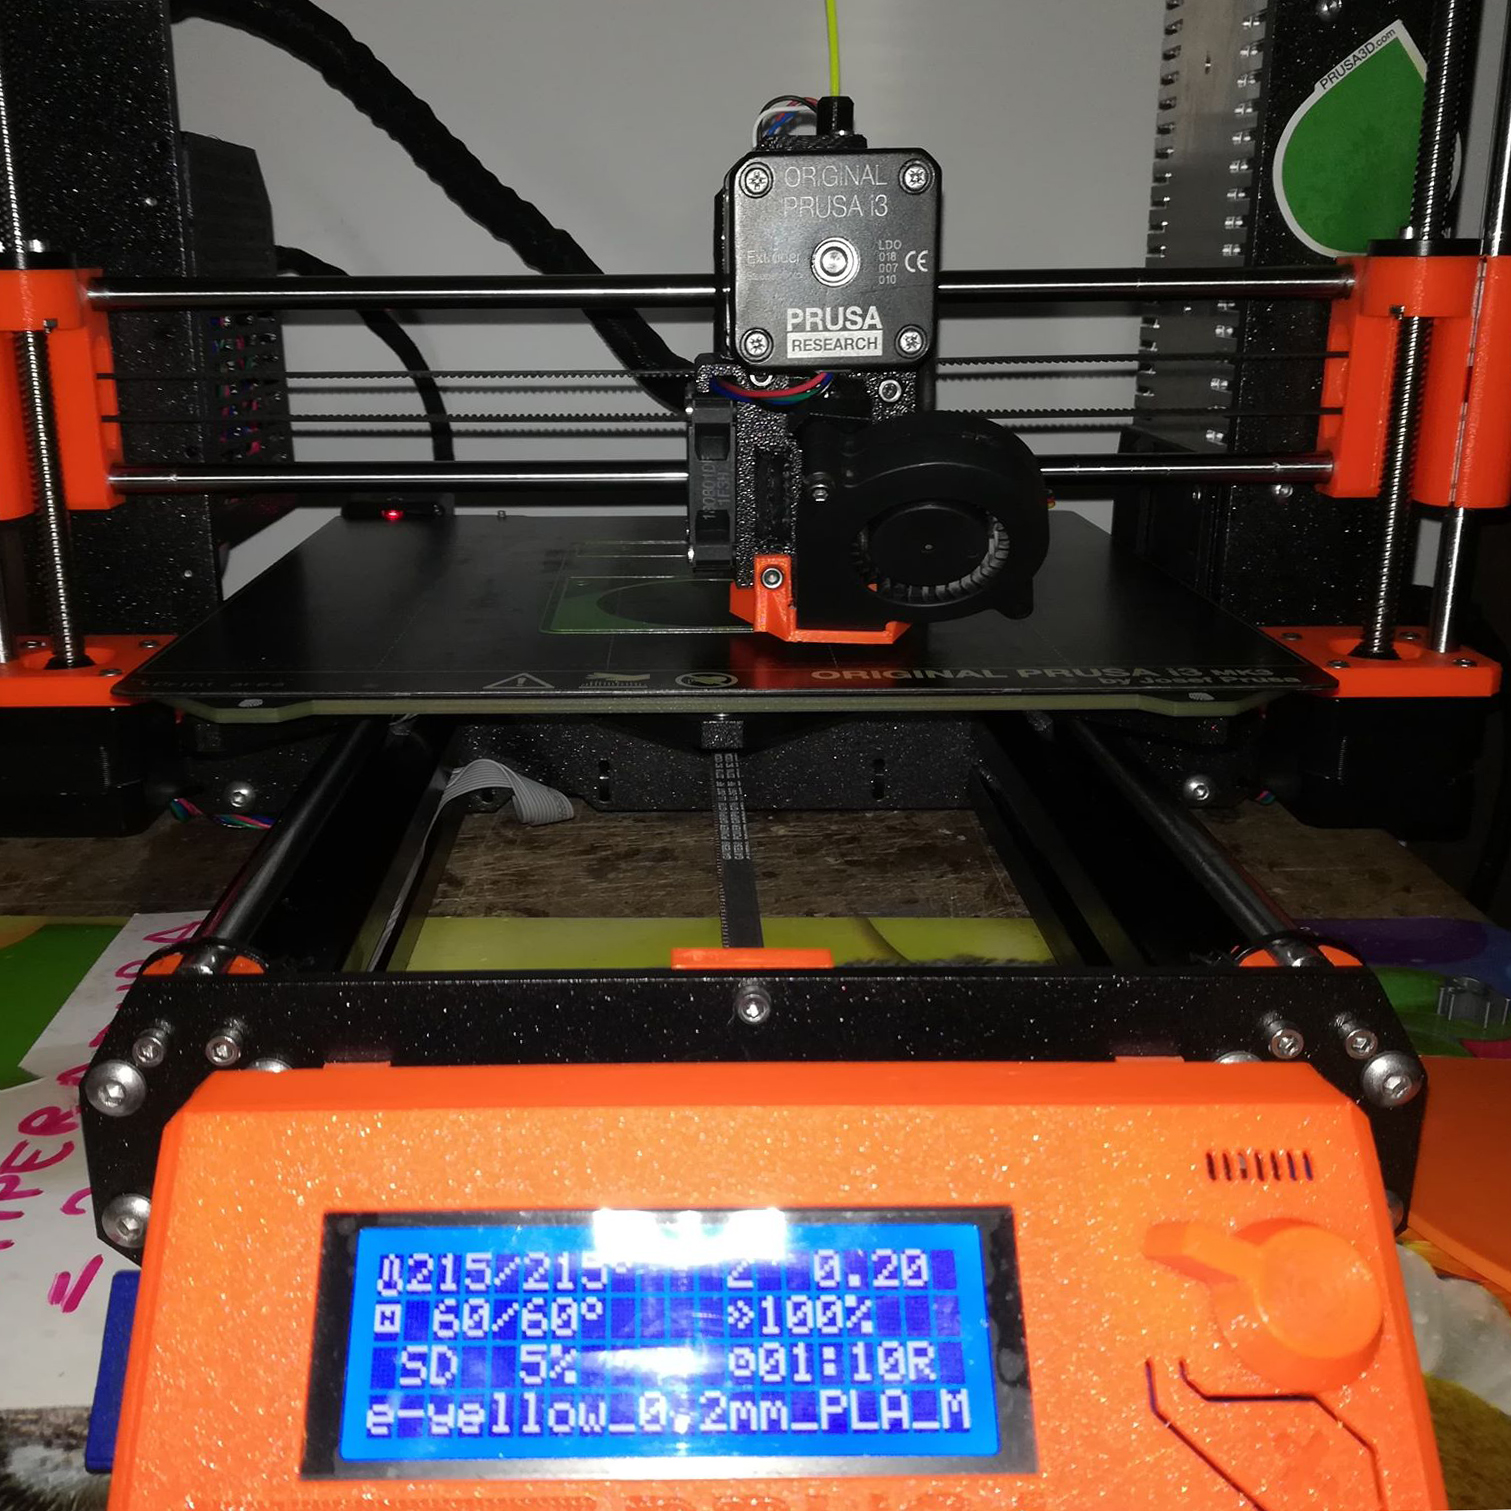
\includegraphics[width=4.8cm]{figures/print1} &
        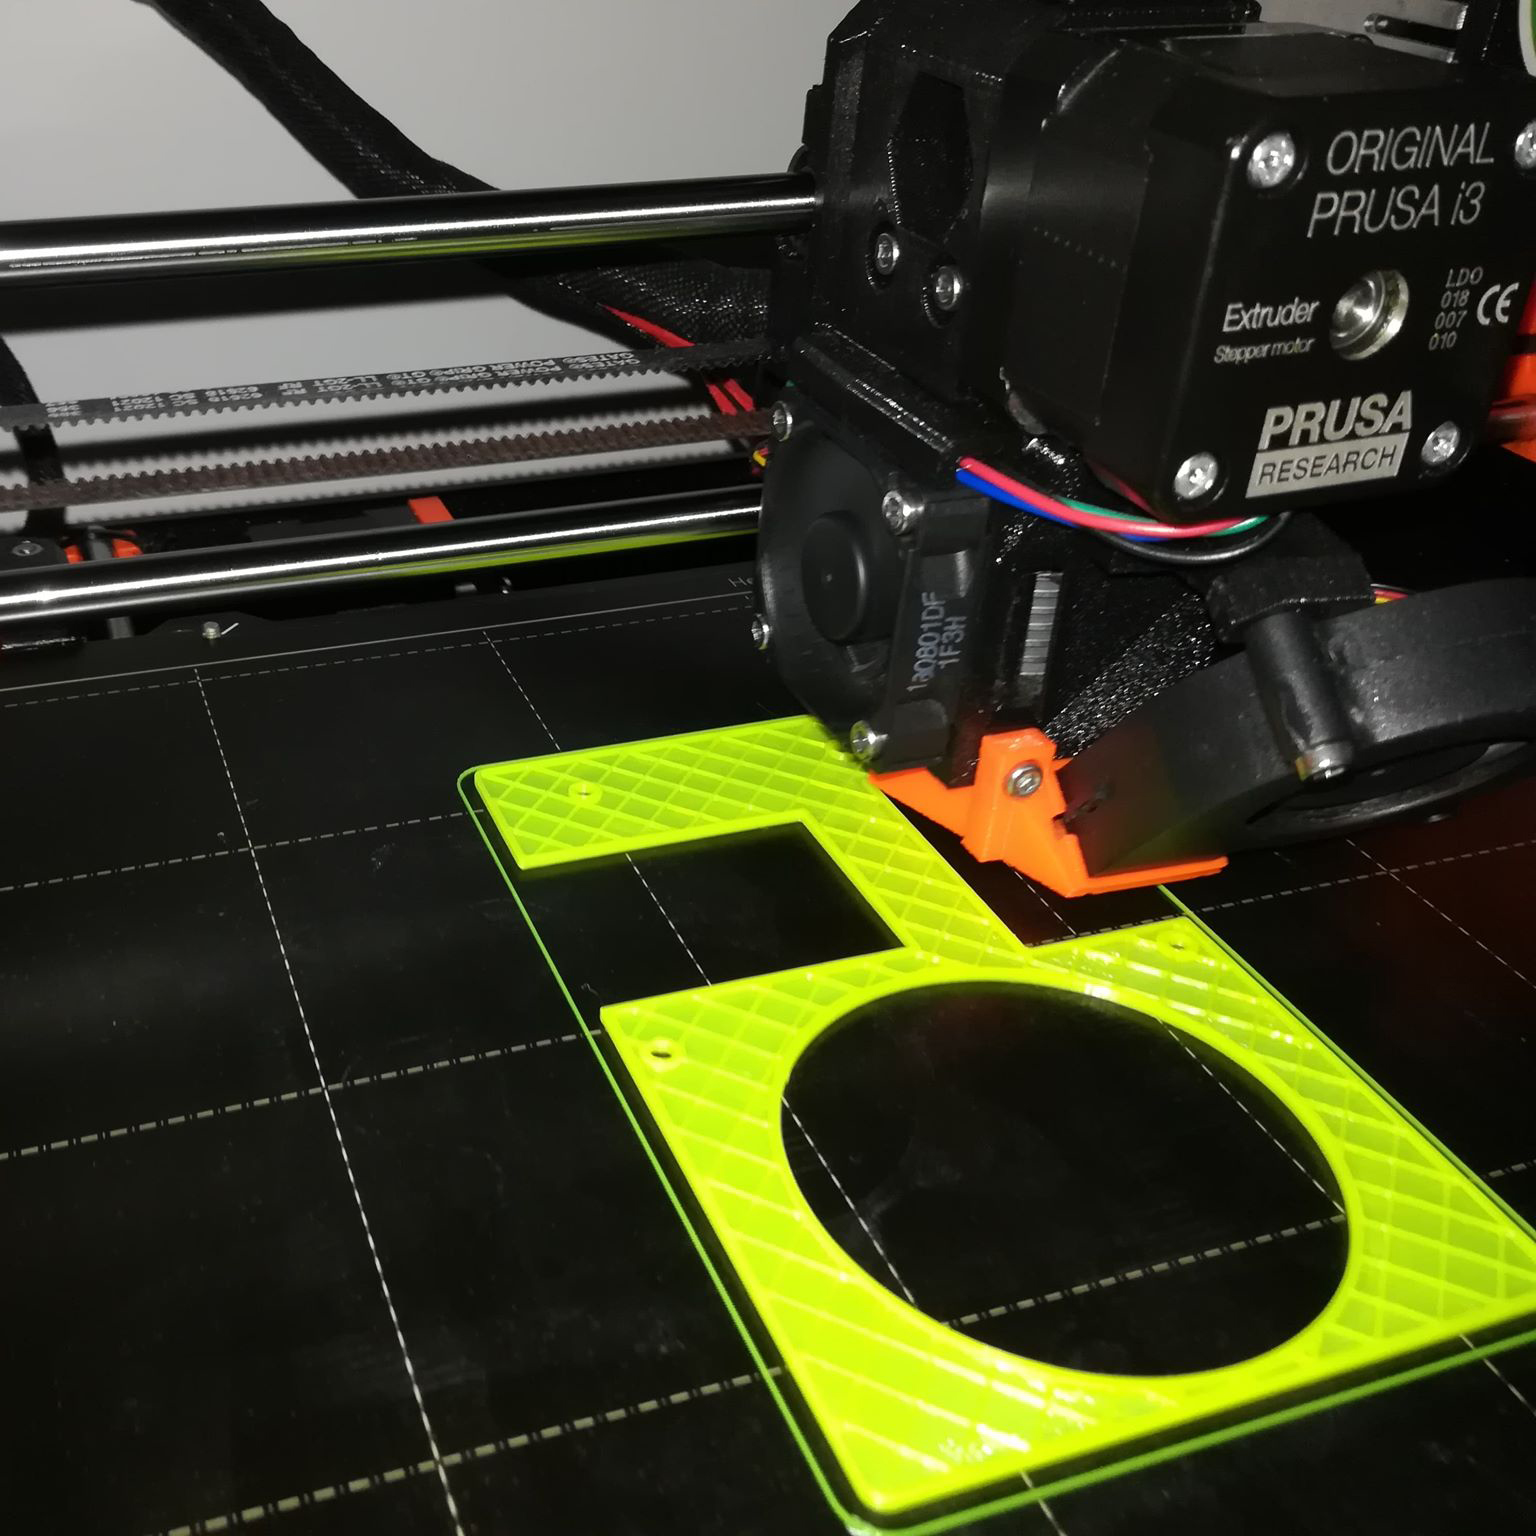
\includegraphics[width=4.8cm]{figures/print3}
    \end{tabular}
    \caption{Printing process on a Prusa I3 MK3S}
    \label{fig:printingTheModel}
\end{figure}

\vspace{0.4cm}\textbf{Edge computing}\vspace{0.4cm}

The objective of Edge computing is to remove the computational burden of IoT caused to Cloud. This layer is represented by the weather station's computer, the Raspberry Pi, which handles some of the computations before sending the messages through the PubSub layer. 

Some of the benefits of having such a layer are summarized in the following:
\begin{itemize}
    \item {data can be pre-processed, cleaned and structured close to the source where data is generated}
    \item {valuable information can be added, such as geo-location information, timestamp, device that originated the event and other potential related information}
\end{itemize}

Although the three-dimensional computer aided design and Edge computing doesn't seem to go hand in hand for too long, they do and there are a couple of reasons for that matter. We found that given an unpredictable environment in which we deploy computing devices, it requires a physical container (digitally designed in my case) to fit the requirements. This physical container will go through a series of refactoring phases until it perfectly fits its purposes. One of the reasons for that is the margin of error taken into account while designing, but usually under or overestimated. The environment exposes the materials to a medium governed by physical and chemical reactions, that may easily destroy the devices. 

As we briefly discussed in the introduction, these are many applications that may benefit from the series of tools and methods exposed in this paper. The ultimate intent of creating a prototype is being manually tested by people, telling us how valuable a product is to the end user. Due to the nature of this project, we were the only one involved in direct contact with the model in terms of testing, but the value of the first prototype quickly dropped after group discussions with faculty colleagues which took a chance at expressing their concerns. 

\vspace{0.4cm}
\textbf{Weather station prototype}
\vspace{0.4cm}

During the initial phase of development, a consistent challenge was approximating the margin of error for the components that were printed with a Prusa research MKi3 printer, such that they could be later connected easily. We determined that a sufficient margin of error would be 0.25mm on each of the joint faces. We will provide an example of our trial and error experience while trying to tailor a prototype for this project. We approached the problem with an naive approach, using power tools, drawing paper and textile materials, during many iterations until reaching the final shape, size and configuration (see Figure \ref{fig:prev}). Both models were designed from scratch by me and can be found in the annexes to the document. Only the second model, depicted in Figure \ref{fig:marker}, will be taken into consideration for further references.

\begin{figure}[htp]
    \centering
    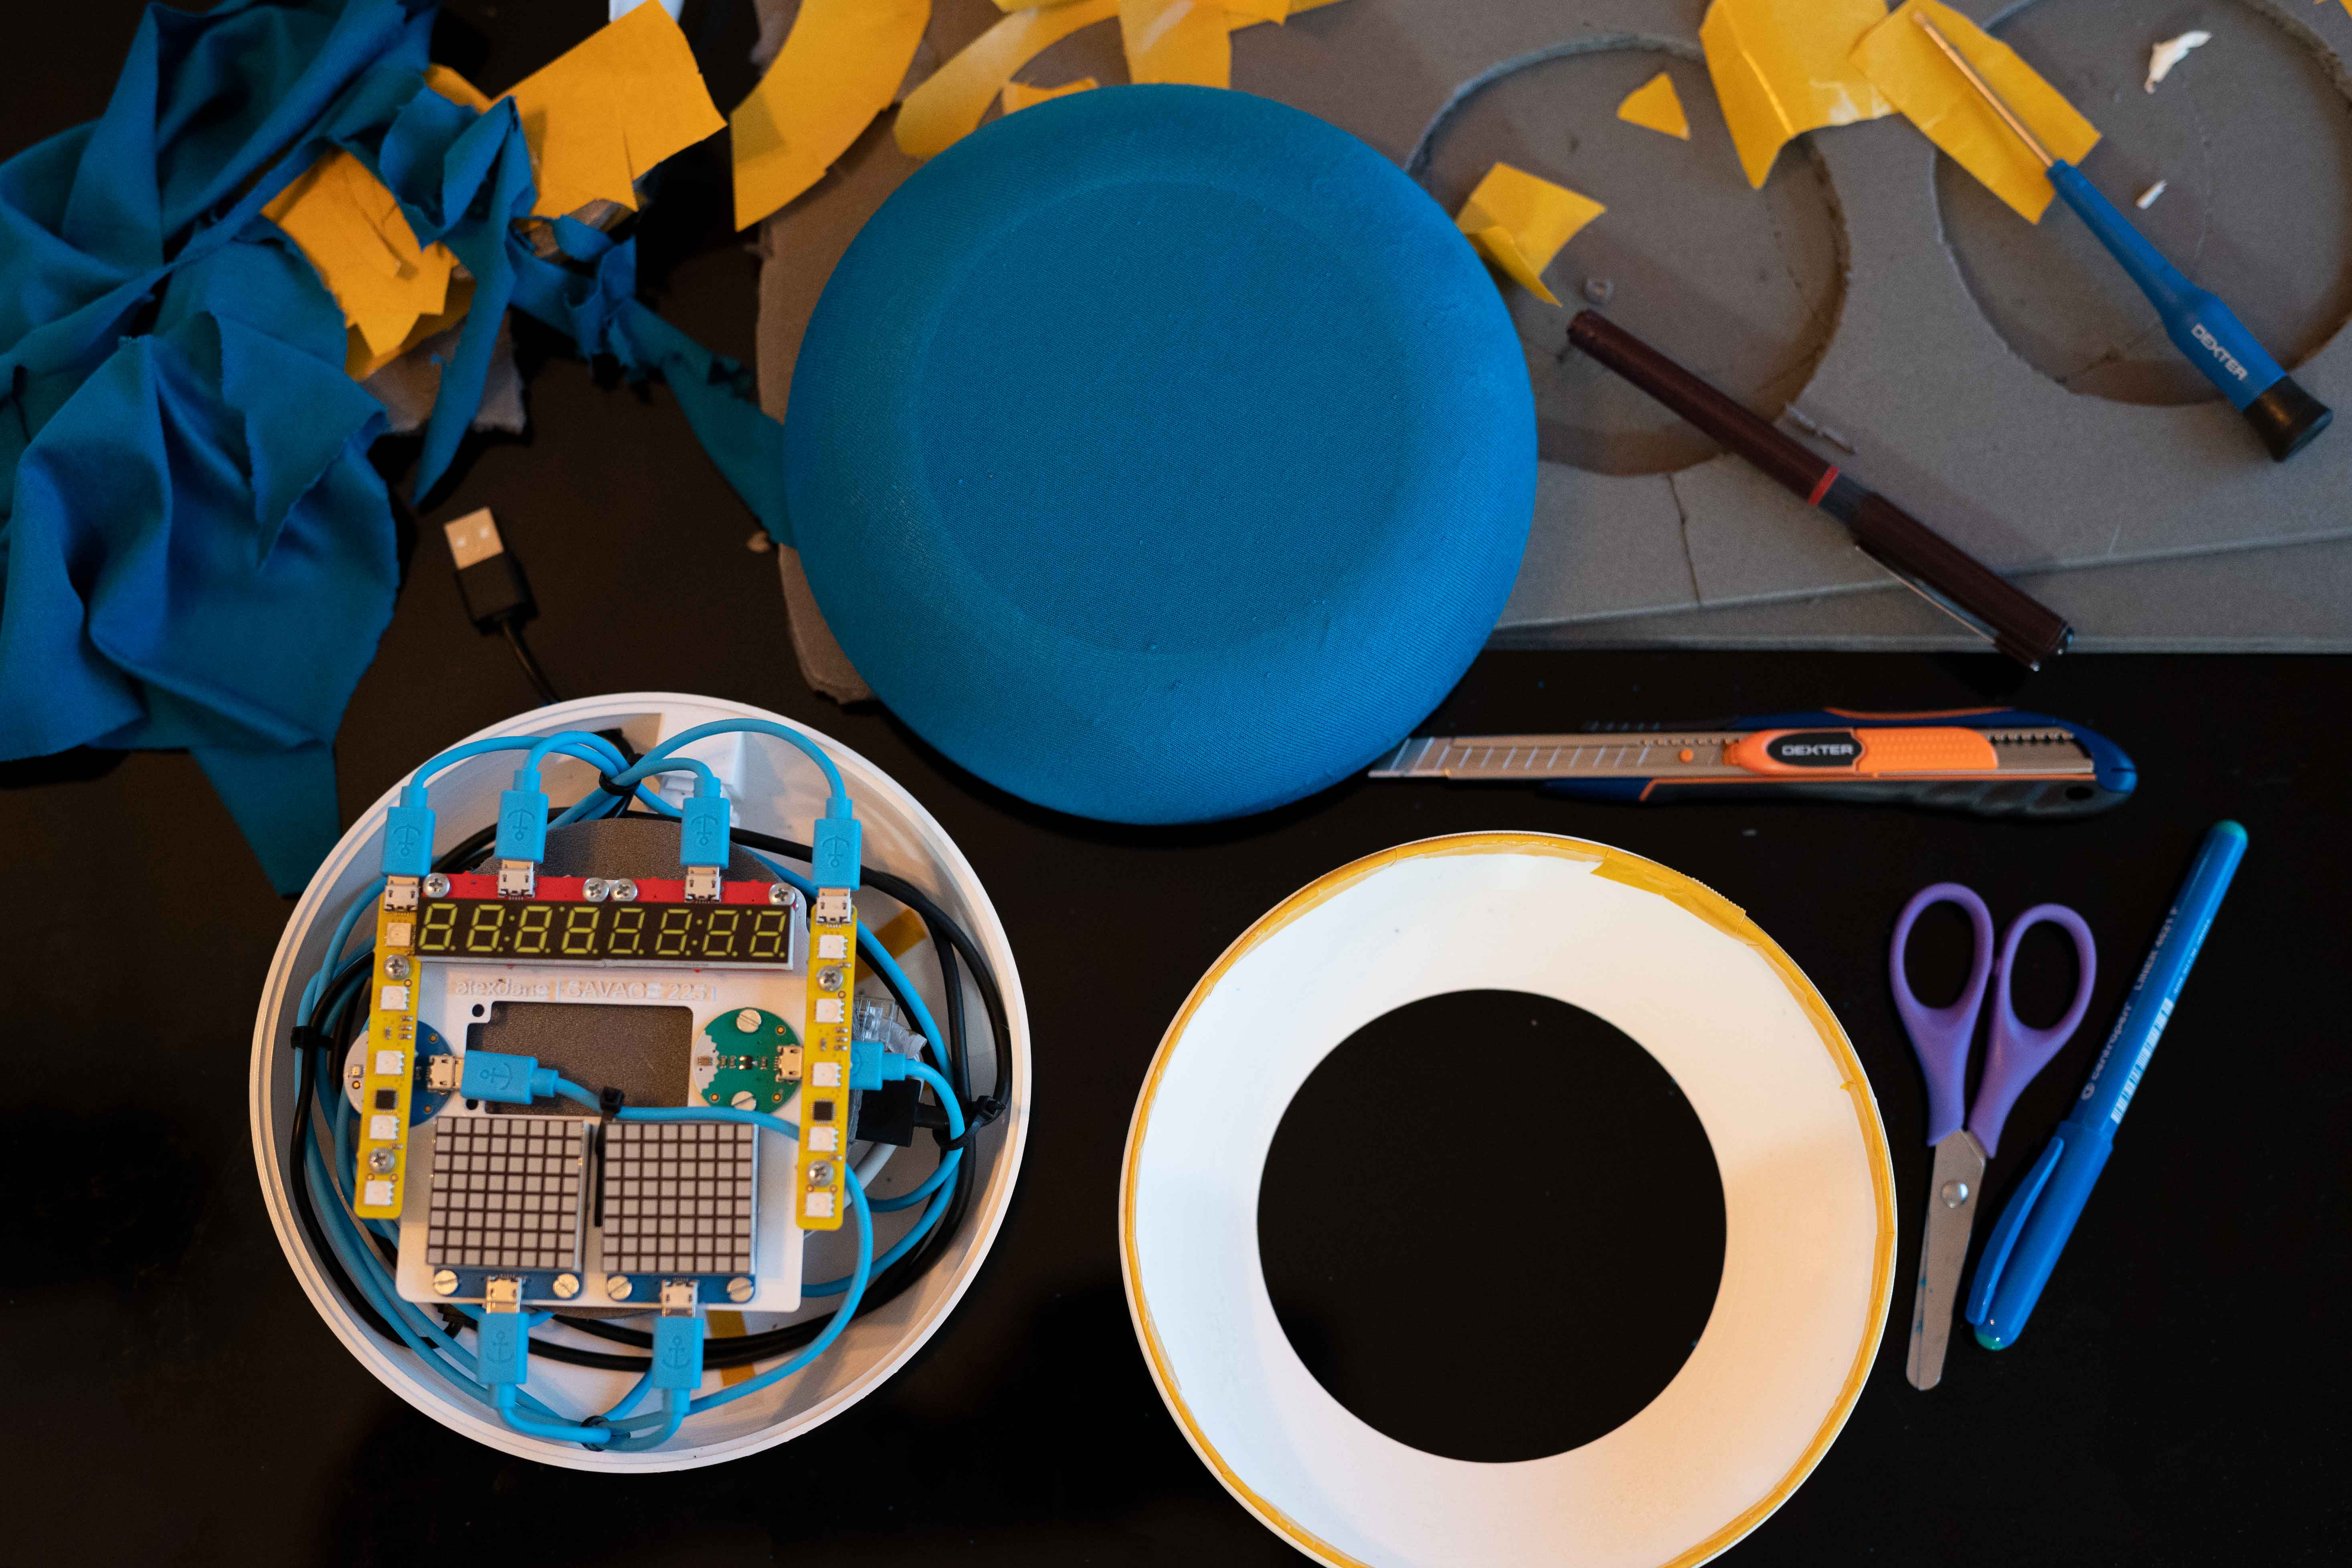
\includegraphics[width = 14cm]{figures/prev_prototype}
    \caption{Prototyping process}
    \label{fig:prev}
\end{figure}

\vspace{4mm}
Key design improvements we made since the first iteration:
\begin{itemize}
    \item{simplify the design, better approximate the errors and reduced the amount of material and the price point by a factor of t\%}
    \item{make it modular and quickly adaptable to changes}
    \item{took the assembly process into consideration from the design phases running simulations of the assembly process before printing it}
    \item{adapt the design to incorporate easily accessible hardware components as opposed to ones sold only in specialized hardware stores}
\end{itemize}

The Figure \ref{fig:schematics} represents a drawing schematics obtained from the digital model, using the Autodesk Fusion 360. The final result is depicted in the Figure \ref{fig:marker}

\begin{figure}[!htb]
    \centering
    \begin{tabular}{ccc}
        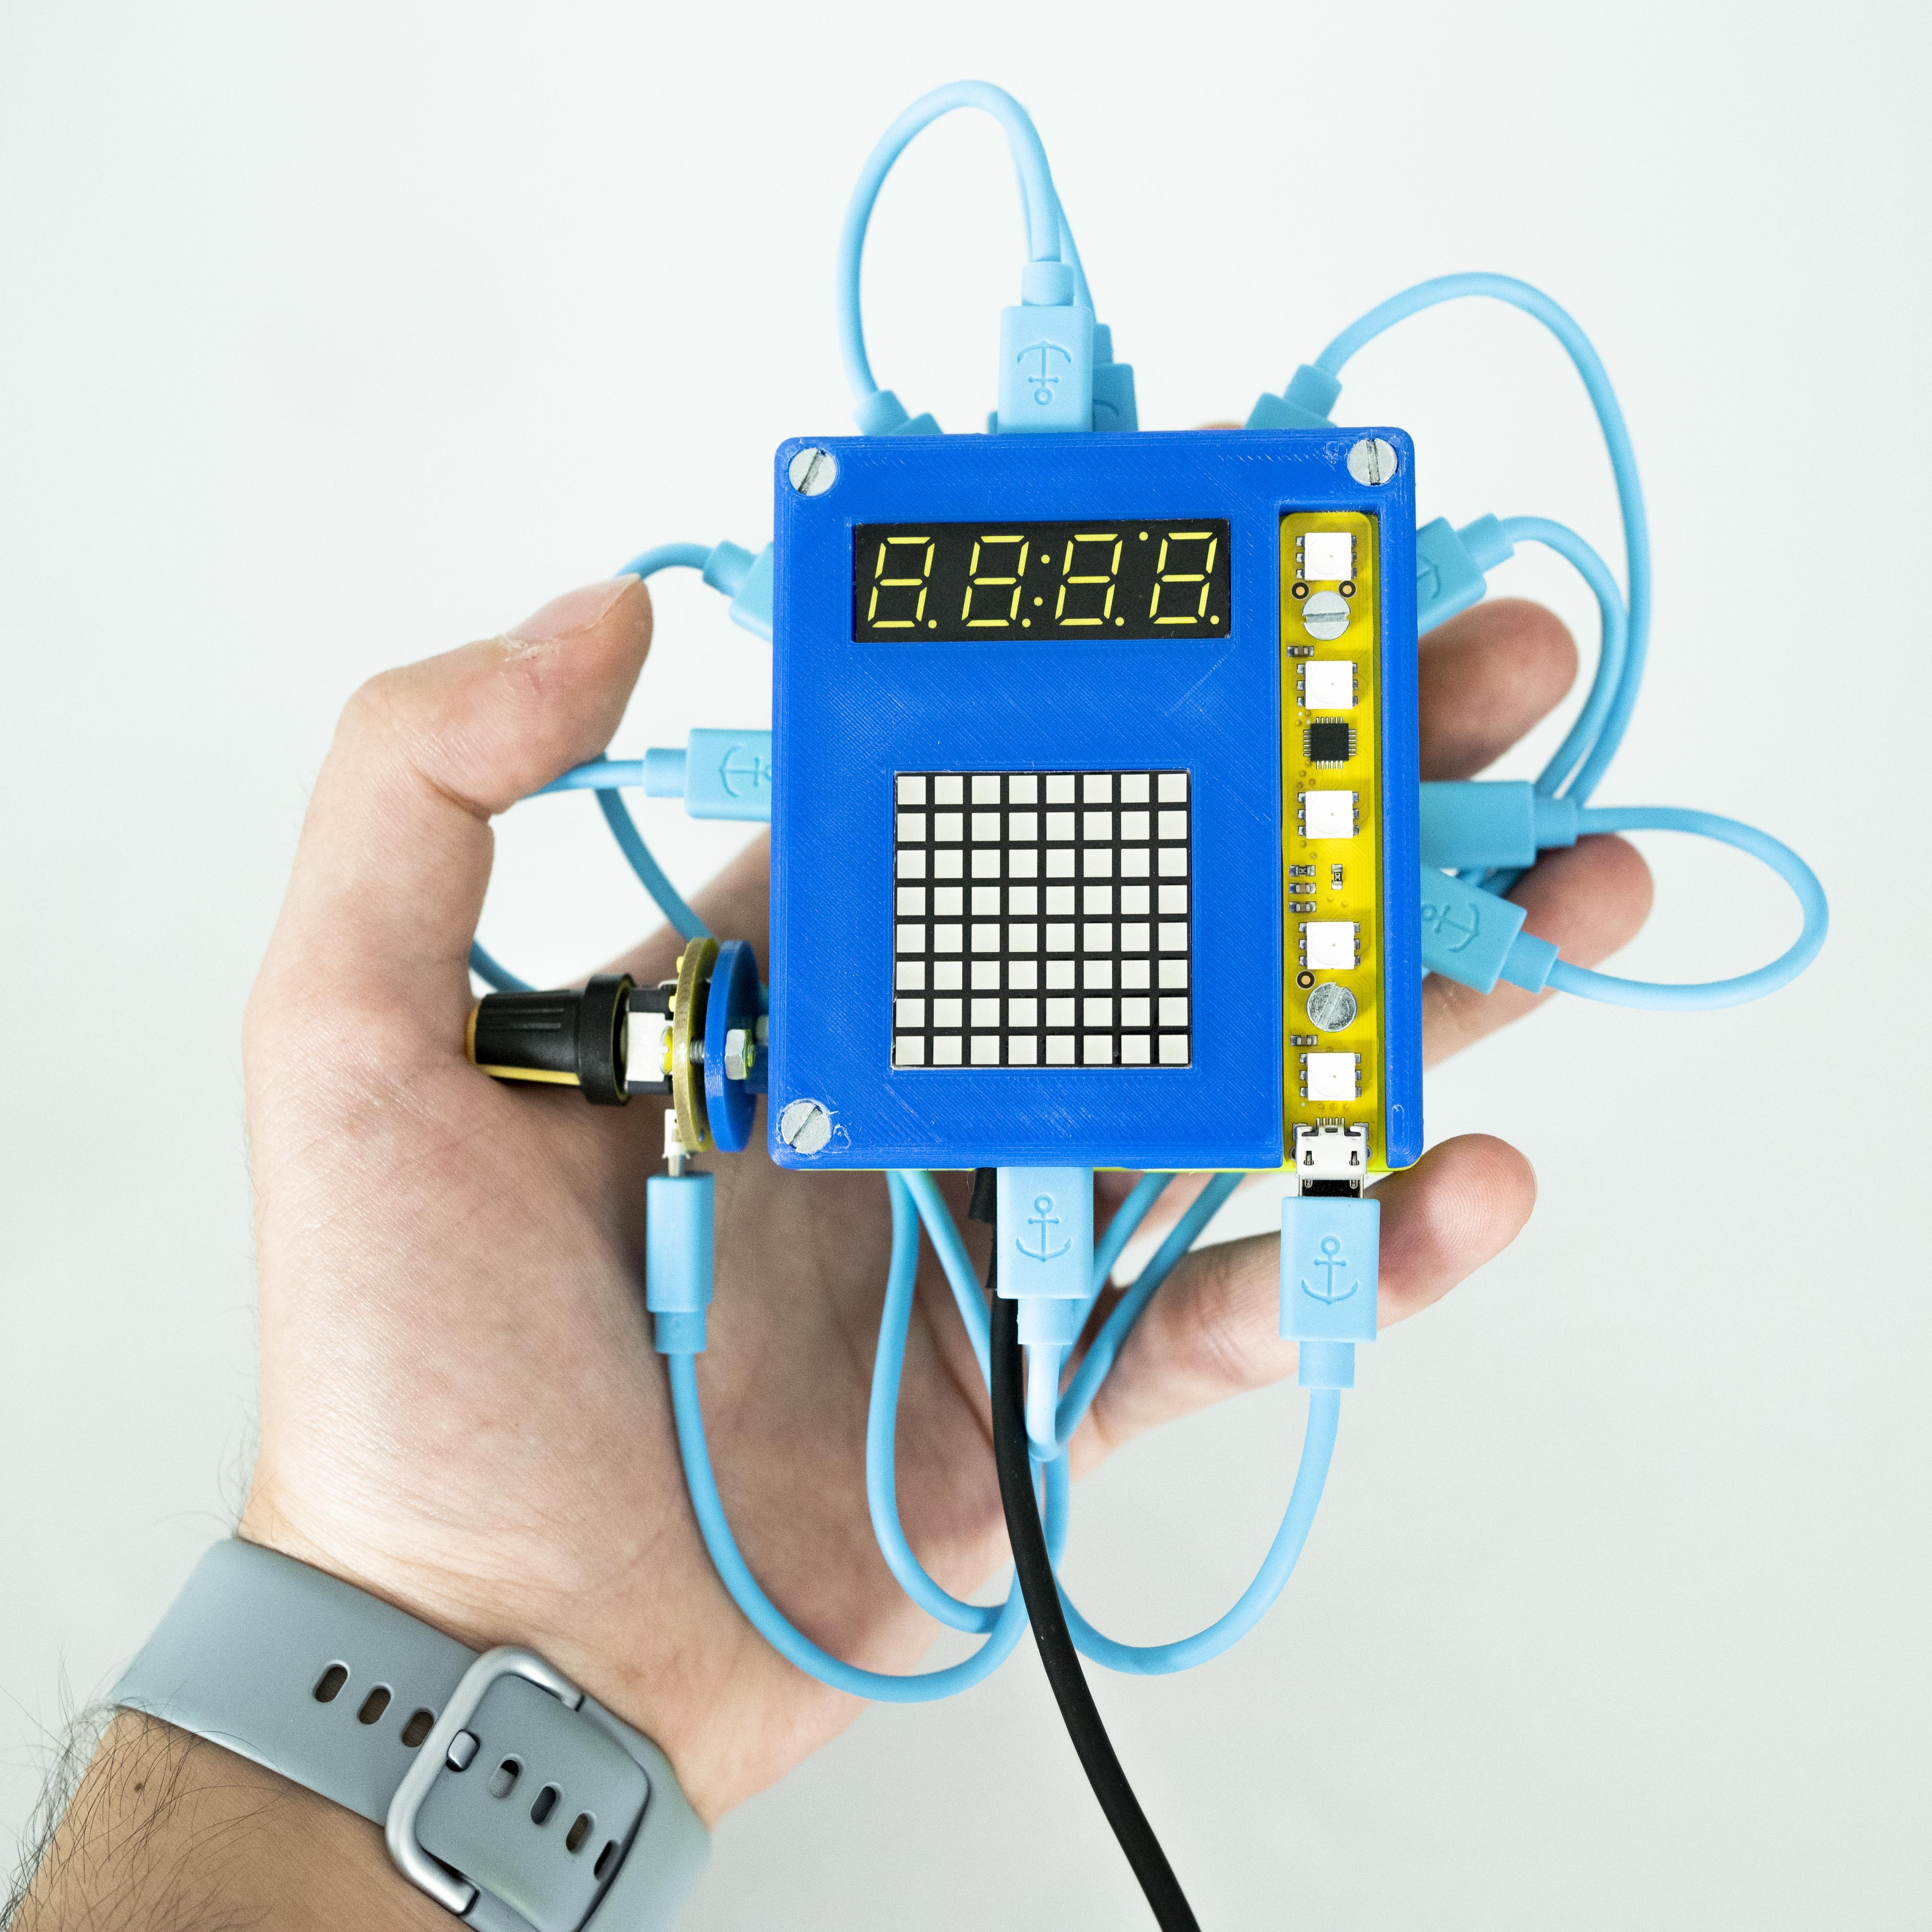
\includegraphics[width=4.8cm]{figures/FRO_3149} &
        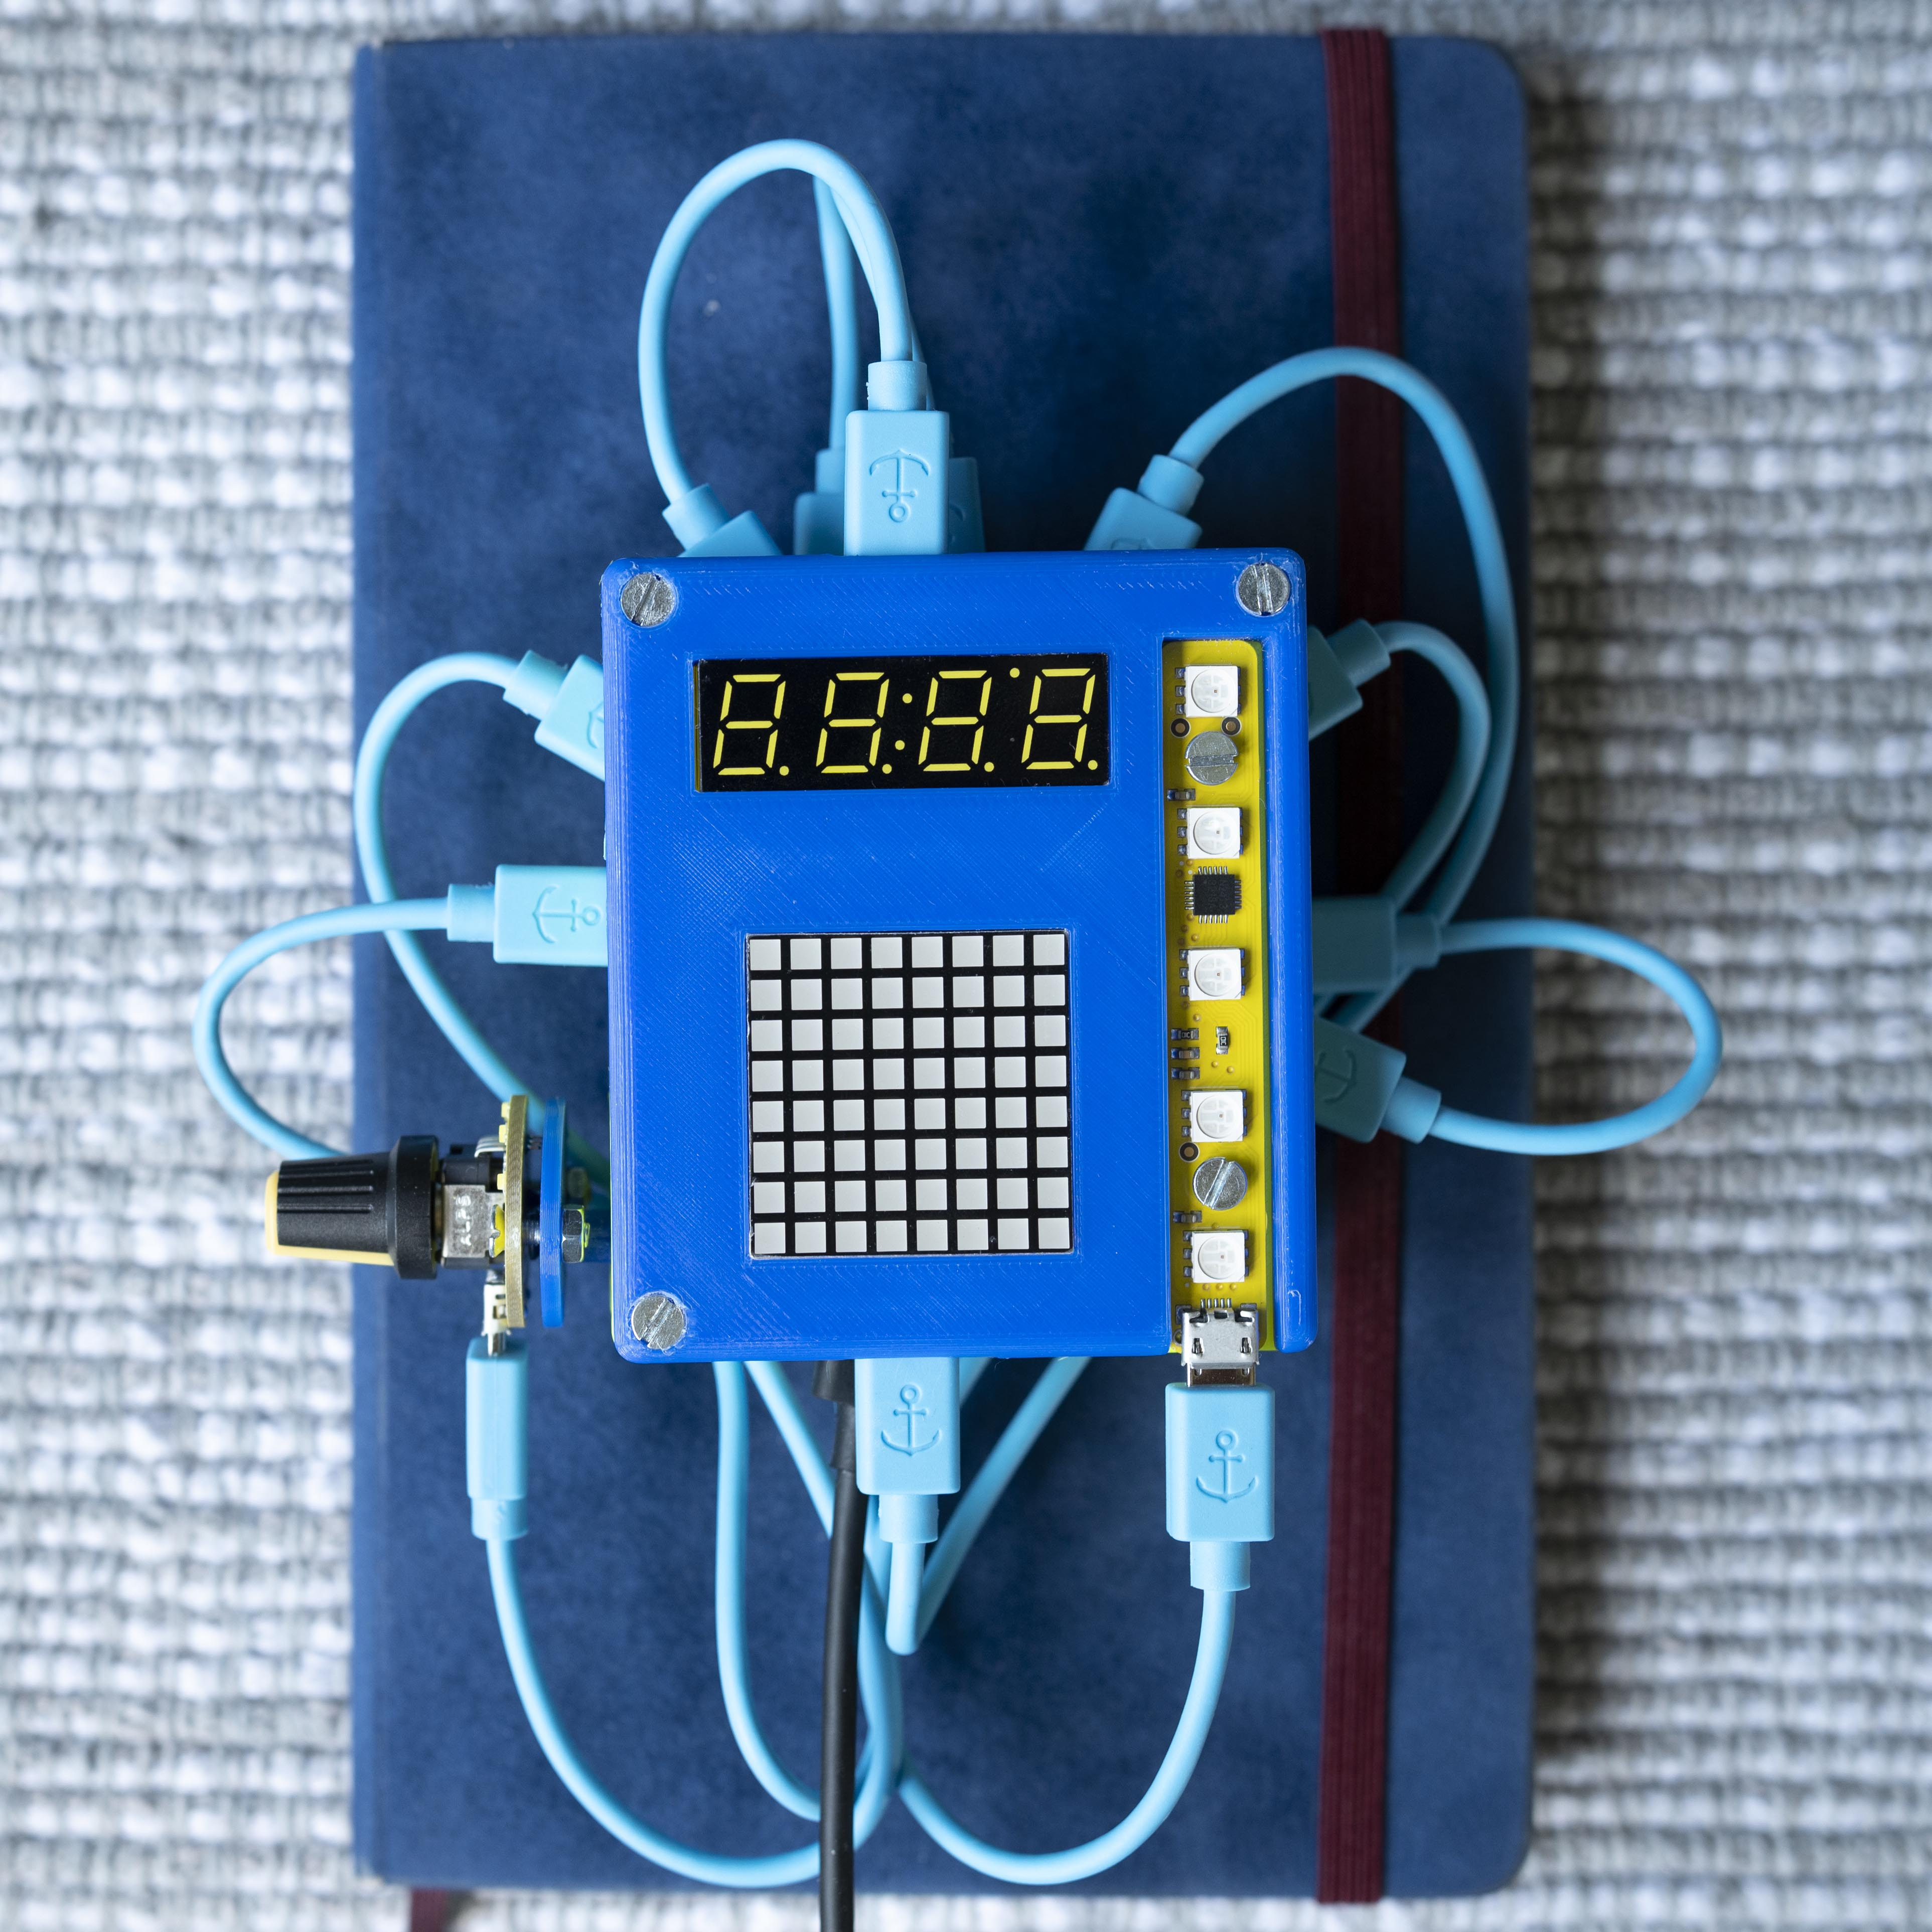
\includegraphics[width=4.8cm]{figures/FRO_3155} &
        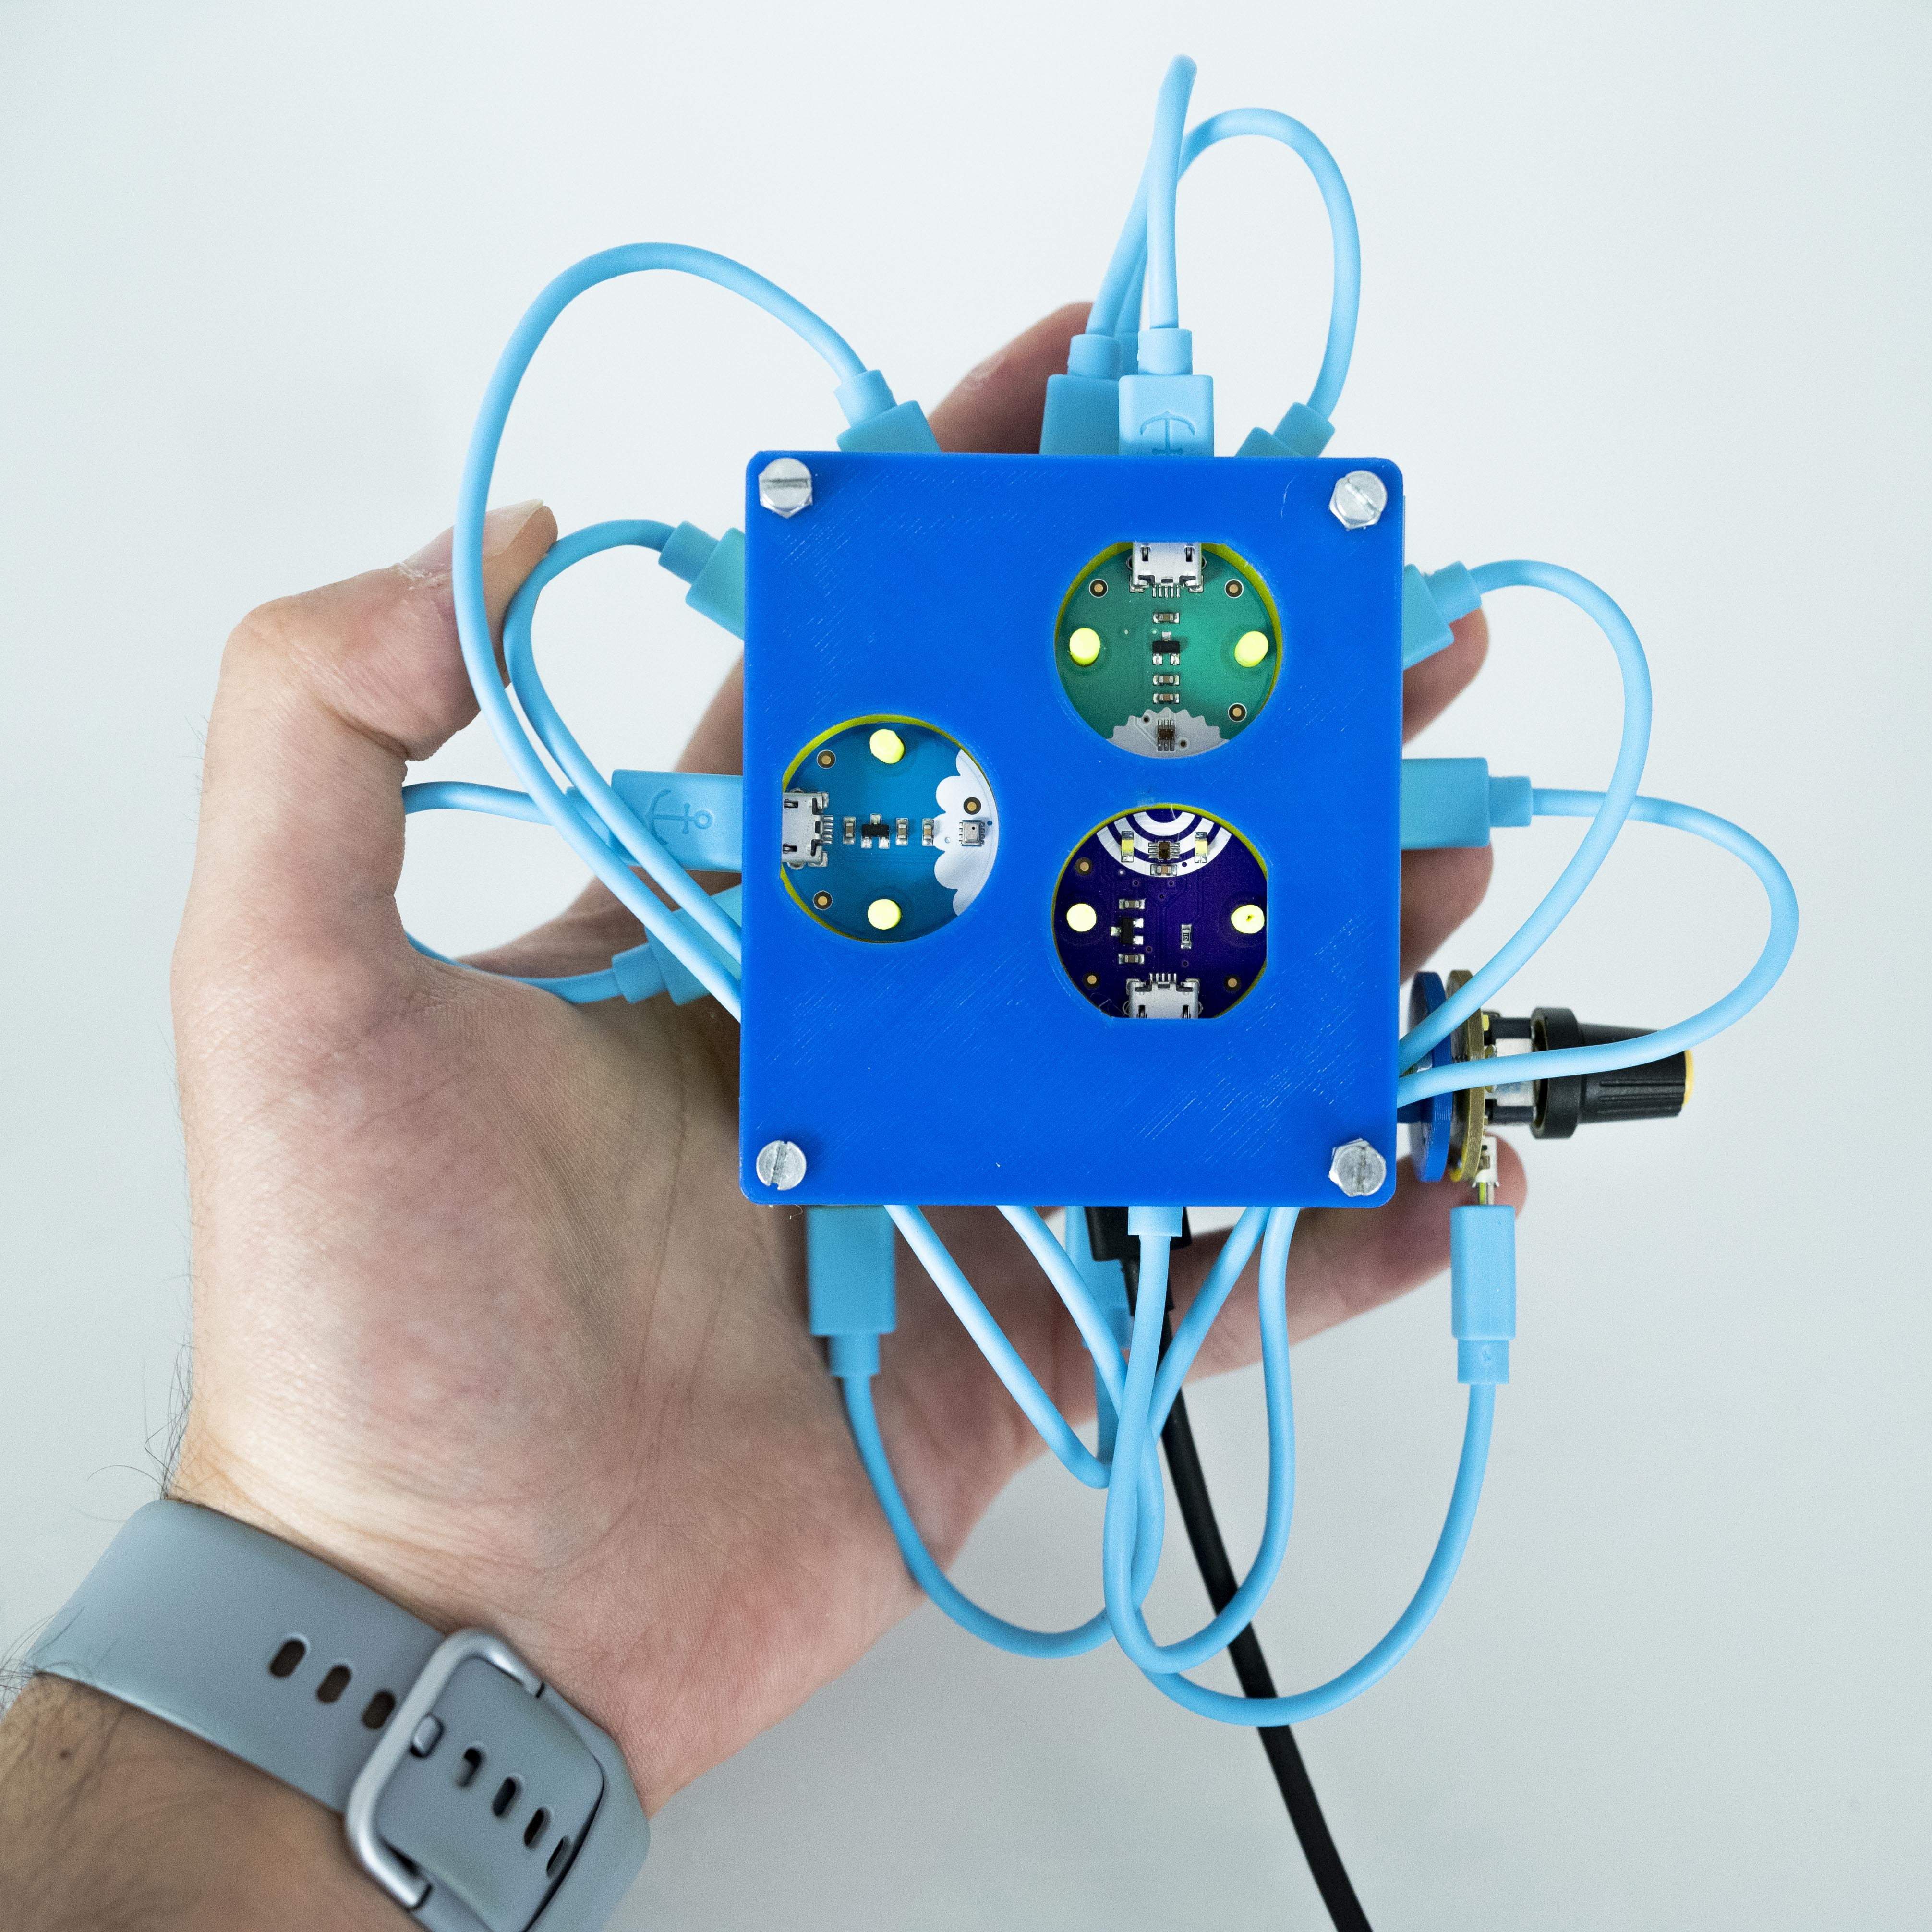
\includegraphics[width=4.8cm]{figures/FRO_3151}
    \end{tabular}
    \caption{Weather monitor prototype}
    \label{fig:marker}
\end{figure}

\section{Google Cloud Platform}

With an e-commerce platform and data lake project, German wholesale giant and food specialist METRO is using Google Cloud Platform to help its customers take more advantage of digital possibilities. Being involved in a 4-month project organized by Metro Systems in collaboration with the Babes-Bolyai University, we had the chance to see first hand one of Google Cloud's case studies \cite{googleCloudUseCase}.

Google Cloud Platform was launched 12 years ago, on April 7, 2008. It initially came up with a number of big data solutions throughout which we will mention: Cloud Dataflow and Pub/Sub. \cite{GoogleCloudPlatform} After a limited testing period in 2010, BigQuery was generally available in November 2011 at the Google Atmosphere conference. The Google Cloud Platform (GCP) is a suite of cloud services hosted on Google's infrastructure. From computing and storage, to data analytics, machine learning, and networking, GCP offers a wide variety of services and APIs \footnote{Application Programming Interfaces} that can be integrated with any cloud-computing application or project. 

We spent a lot of time reading about Google Services, where a couple of things kept us hooked, wanting to know more. If you ever used one of Google's services, like Gmail, you may very well agree that they have meticulously designed their products. So, it made me wonder - what if the process of streaming, analyzing data and building an application has the same familiar and intuitive experience we already experienced with other tools. Besides that, we were searching for an accessible programming language and found that we can code in Python or Go. We can think of Python's versatility as one reason for its ongoing popularity throughout students and makers, myself included. In order to learn how to use the platform, you have 300\$ to spend on whatever service you want, depending on the reason that brought you on the platform. Mine was mining data streams, and we found it great to see all the Big Data services in one place so that we can read about each individual one. The price point for Big Data services is considerably lower than other services we found while researching.

\begin{table}[h!]
  \begin{center}
    \label{tab:table2}
    \begin{tabular}{l l l} % <-- Alignments: 1st column left, 2nd middle and 3rd right, with vertical lines in between
      \textbf{Service} & \textbf{Feature} & \textbf{Costs}\\
      \hline
        Dataflow & Deploy on Cloud \& Local runners & Streaming worker\\
        & Batch and streaming data processing pipelines & defaults: 4vCPU, 15GB \\
        & Apache Beam programming model & memory, 420GB Disk\\
        & & costs \$0.09/hour \\
      \hline
    % \vspace{4mm}
        PubSub & Data streaming from various processes or devices & The first 10 gigabytes \\
        & Distributing event notifications & of usage are free. After \\
        & Low cost & that, the price for \\
        & & ingestion or delivery of \\
        & & messages is \$40 per TiB \\
      \hline
    % \vspace{4mm}
        BigQuery & Real-time analytics on streaming data & Storage API: \$1.10/TB \\
        & Fuly managed and serverless & Streaming inserts: \$0.01 \\
        & Built-in ML and GIS & /200MB; Queries \\
        & High speed, in-memory BI & on demand: \$5/TB \\
    \end{tabular}
    \caption{Features and costs service analysis extracted at 17 Apr 2020}
  \end{center}
\end{table}

There are three big vendors of public cloud computing solutions, Amazon, Google and Microsoft. The cloud computing market is expected to hit \$760.98 billion by 2027 \cite{market_cloud}. Depending on the report you read, Google is either the third or the fourth largest public cloud vendor, behind Amazon, Microsoft and (possibly) IBM. While the other competitors increased the number of services included in their portfolio, Google has a narrower focus and specializes in meeting the needs of developers. Unlike Amazon and Microsoft, which approached the cloud with IaaS \footnote{Infrastructure as a service} solution, Google's first public cloud service was its PaaS \footnote{Platform as a service}, called App Engine. App Engine first launched as a private preview for developers in April 2008, then it was made public in May, criticised for some of its shortcomings that were solved in 2009, and followed by Cloud Storage in 2010. Google isn't competing on existing solutions, but finding its own slice in this market, offering some specialized tools for developers that are hard to find elsewhere.

How did other companies have successfully managed to integrate Google's services into their business model? At Spotify, the strategy was to outsource time consuming problems that are not core to their business to Google and GCP \cite{SpotifyLabs1}. Particularly, to take advantage of managed messaging queues, data processing, and storage. Also, in terms of warehousing, BigQuery's high-speed streaming insertion API provides a powerful foundation for real-time analytics, making the latest business data immediately available for analysis. "We can also leverage Pub/Sub and Dataflow to stream data into BigQuery. The backbone of our system is Cloud Pub/Sub." \cite{SpotifyLabs2} 

\begin{figure}[htp]
    \centering
    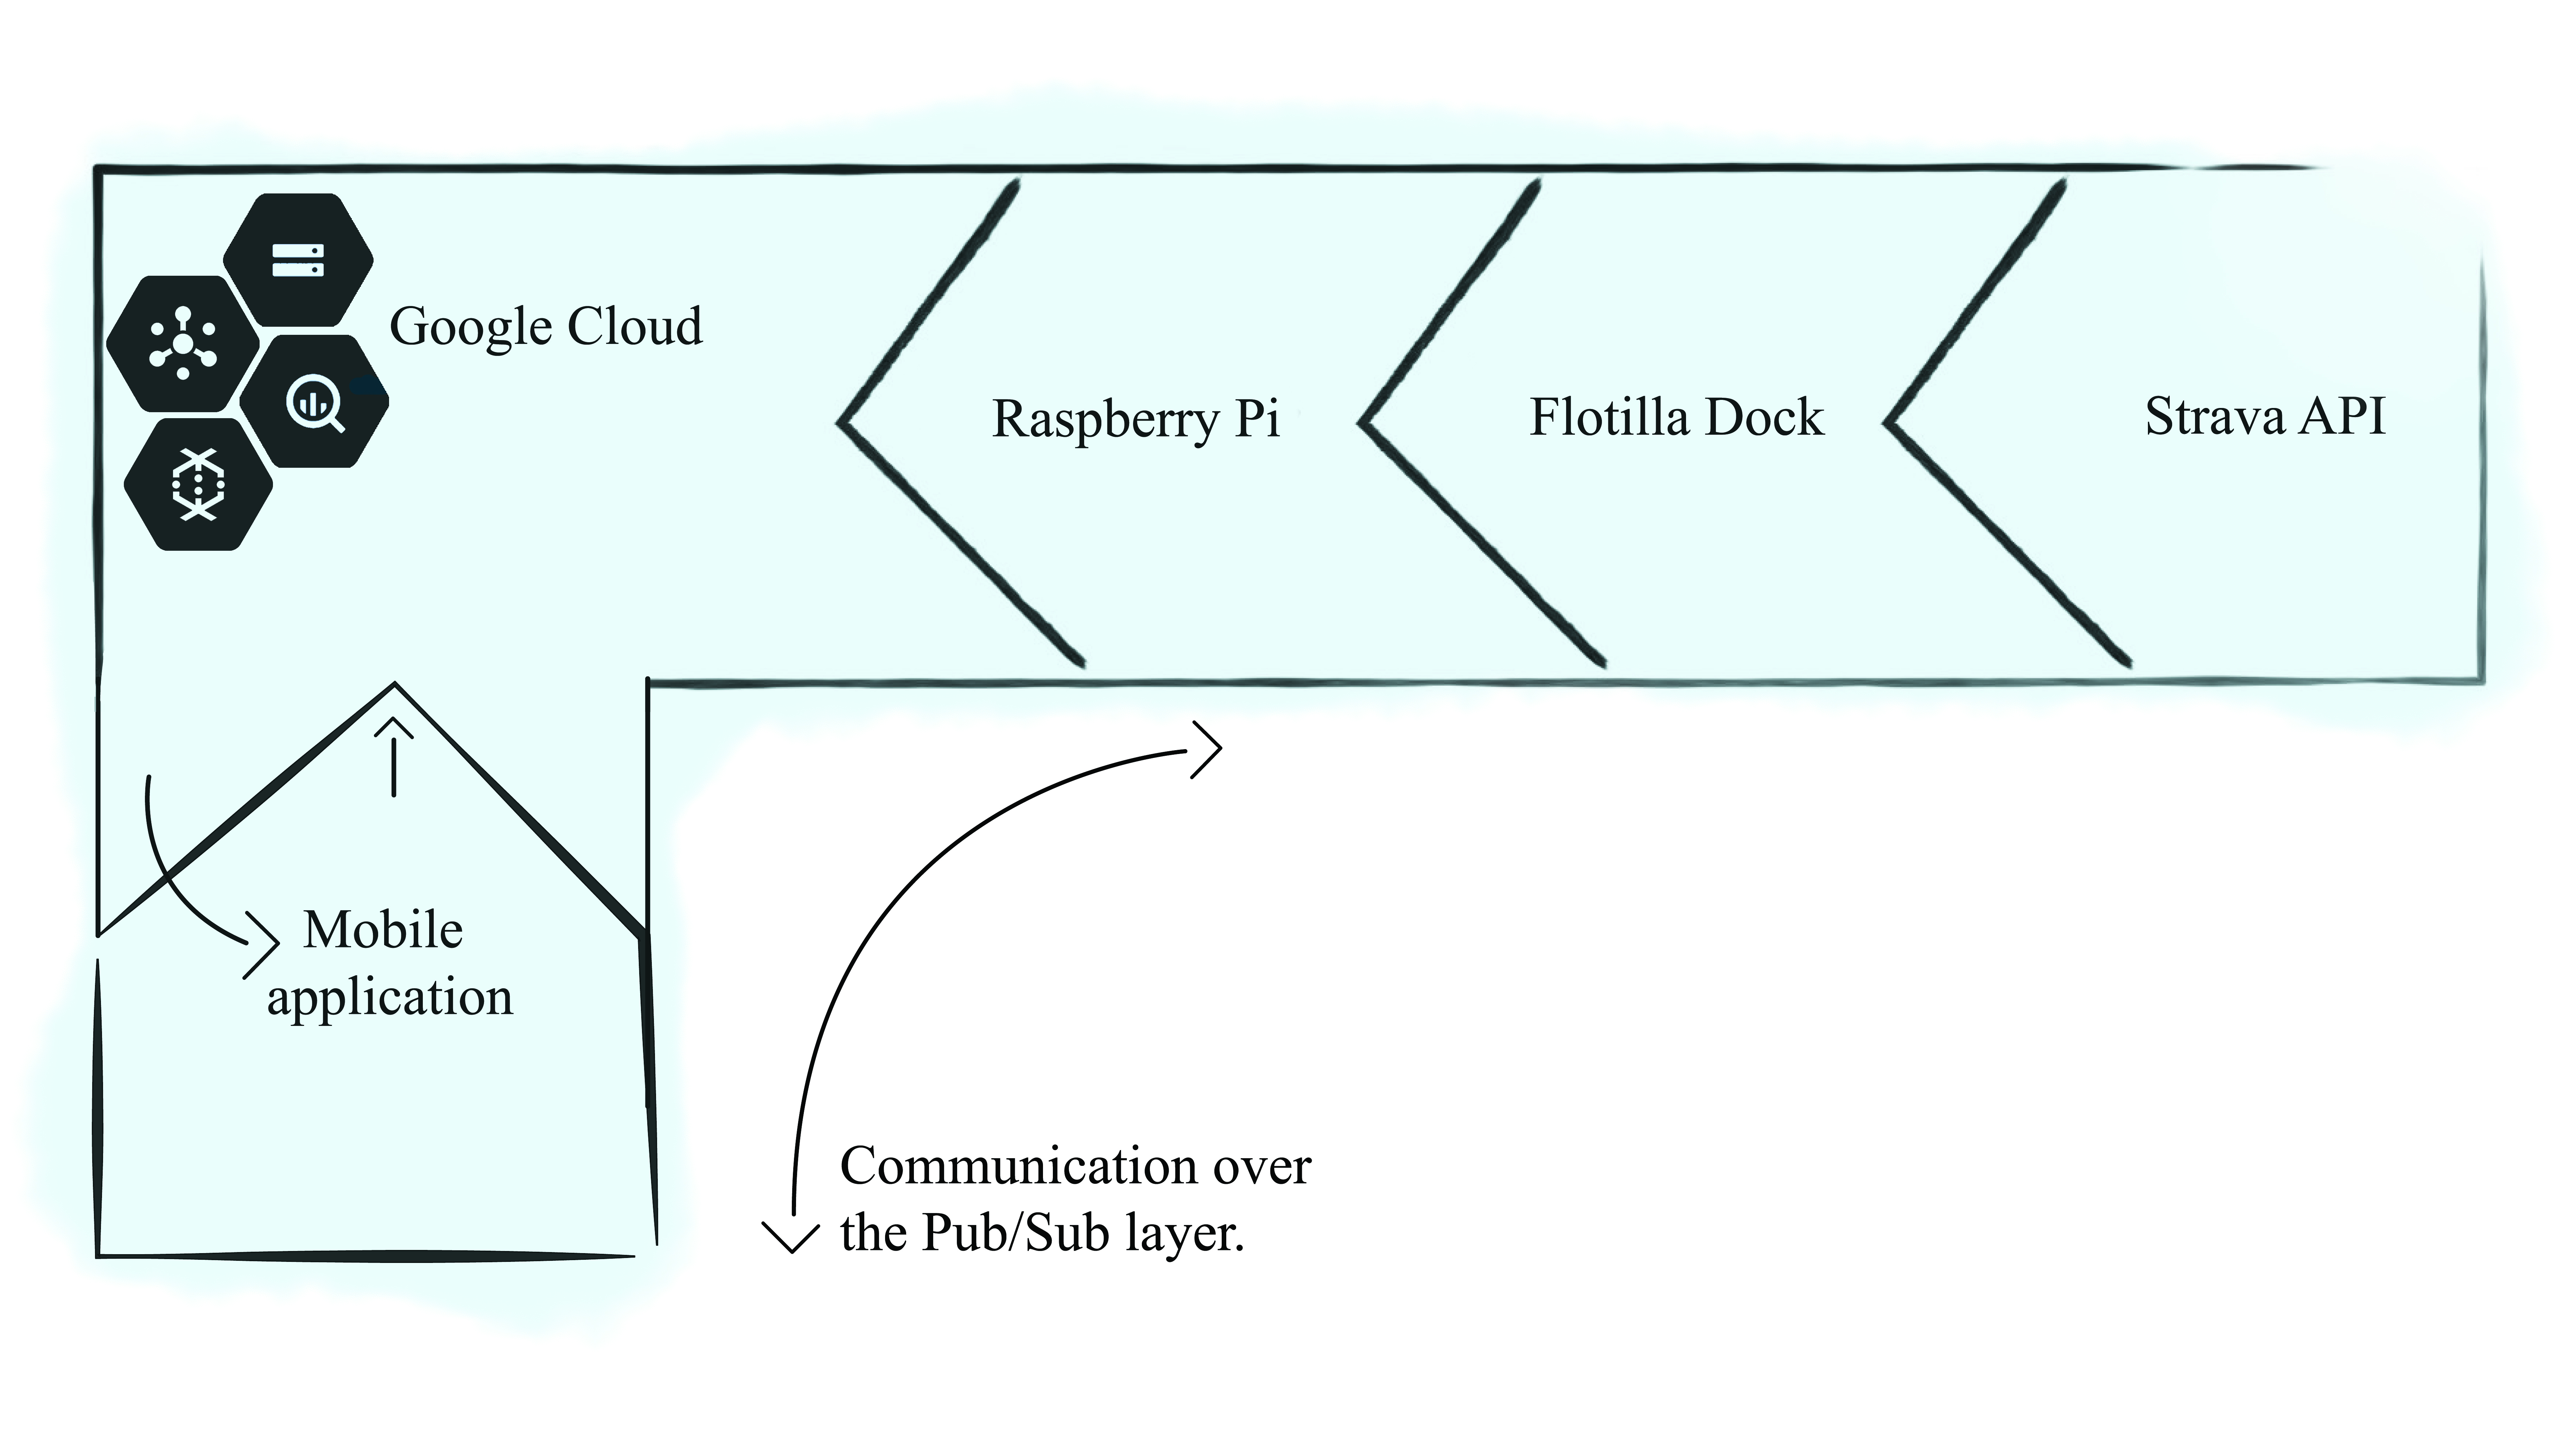
\includegraphics[width = 12cm]{figures/architecture_large_scale}
    \caption{Large scale architecture}
    \label{fig:lsa}
\end{figure}

\subsection{Cloud Dataflow}

Google Cloud Dataflow is one of Beam's supported distributed back-ends data processing pipeline systems that we can program against in Python, Java or Go. During this paper you will find the notion of data flow under different contexts, so it is worthwhile exploring the differences. There is a Cloud Dataflow, which is a service meant to run the ETL process. It is also the name of a model proposed by Google in a paper we'll discuss later on. Additionally, data flow can be used with its most common definition, as the abstraction of data transfer between two points.

The following sections are dedicated to the backbone models used over the years and more recently by Google in Cloud Dataflow. They are not directly influencing the project, yet we found them worth exploring.

\subsubsection{The Apache Beam programming model}

Beam started as a Google project with interests in the area of making data processing easier, faster and with a lower price point. The Beam model is a direct successor to MapReduce, FlumeJava, and Millwheel inside Google and is focused on providing a unified solution for batch and stream processing. Such solutions are intended to respond to shortcomings of data processing frameworks such as Apache Spark and Flink. K.M.J Jacobs wrote in one of his reports for CERN, Geneva, Switzerland back in 2016 that Apache Beam is worth investigating when it is released. \cite{7776539} 

Apache Beam is one implementation of the Dataflow model paper. Google released an open SDK implementation of the Dataflow model in 2014 and an environment to execute Dataflows locally (non-distributed) as well as in the Google Cloud Platform service. In 2016 Google donated the core SDK as well as the implementation of a local runner, and a set of IOs (data connectors) to access Google Cloud Platform data services to the Apache Software Foundation.

Beam is a simple, flexible, and powerful system for distributed data processing at any scale. It provides a unified programming model, a software development kit to define and construct data processing pipelines, and runners to execute Beam pipelines in several runtime engines, like Apache Spark, Apache Flink, or Google Cloud Dataflow. Beam can be used for a variety of streaming or batch data processing goals including ETL, stream analysis, and aggregate computation. The underlying programming model for Beam provides MapReduce-like parallelism, combined with support for powerful data windowing, and fine-grained correctness control. \cite{BeamProposal}

Beam was designed from the start to provide a portable programming layer. When you define a data processing pipeline with the Beam model, you are creating a job which is capable of being processed by any number of Beam processing engines. Several engines have been developed to run Beam pipelines in other open source runtimes, including a Beam runner for Apache Flink and Apache Spark. There is also a “direct runner”, for execution on the developer machine (mainly for dev/debug purposes). Another runner allows a Beam program to run on a managed service, Google Cloud Dataflow, in Google Cloud Platform. In the Beam proposal, the authors believe that "submitting Beam as an Apache project will provide an immediate, worthwhile, and substantial contribution to the open source community". \cite{BeamProposal}

\subsubsection{MapReduce model}

One of the old models that represented a base for research is the MapReduce model. It is a programming paradigm for large scale computation across a computing cluster. Google initially came up with this idea of doing large scale computation in the \cite{TheMapReduceModel} in 2003, then it got popularized into an open source implementation called Apache Hadoop. In order to take an example, the job you want to create has to be decomposable in a map phase and a reduce phase. In the map phase we want to do the same computation over the elements of a dataset, and as we do that, all the data is distributed over the cluster, so we want to be able to compute the result depending only on that element. The reduce phase will then take the results of the map phase, reduce it down to kind of a single value, then send it back as the result of the computation. \cite{mapReduceComp}

\subsubsection{Dataflow model}

"As we designed the Dataflow Model, we took into consideration our real-world experiences with FlumeJava and Mill-Wheel over the years. Things which worked well, we made sure to capture in the model; things which worked less well motivated changes in approach." \cite{TheDataflowModel} 

The model has two basic primitive actions: (1) ParDo for generic parallel processing. As you can recall from the MapReduce model, each input element to be processed is provided to a user-defined function which generates an output. (2) GroupByKey is key-grouping (key, value) the intermediate results of the ParDo function. Aside from those, the model includes windowing techniques, triggers, and incremental processing. It was internally implemented in FlumeJava \footnote{A Java library that makes it easy to develop, test, and run efficient data parallel pipelines} with MillWheel used as the underlying execution engine for streaming mode. Additionally, an external reimplementation for Cloud Dataflow was made available.

\vspace{0.4cm}
\textbf{Core concepts}
\vspace{0.4cm}

The Beam programming model has been designed with simplicity, scalability, and speed as key tenants. In the Beam model \cite{BeamProposal}, you only need to think about four top-level concepts when constructing your data processing job:

\begin{itemize}
    \item{Pipelines - The data processing job made of a series of computations including input, processing, and output}
    \item{PCollections - Bounded (or unbounded) datasets which represent the input, intermediate and output data in pipelines}
    \item{I/O Sources - APIs for reading and writing data which are the roots and endpoints of the pipeline}
\end{itemize}

\subsection{Cloud PubSub}

Pub/Sub is a message-oriented middleware hosted by Google in the cloud that provides a scalable, durable event ingestion and delivery system that serves as a foundation for modern stream analytics pipelines. It provides many-to-many asynchronous messaging among independent written applications. In Cloud Pub/Sub, publisher applications and subscriber applications connect with one another through the use of a shared string called a topic. A publisher application creates and sends messages to a topic. Subscriber applications create a subscription to a topic to receive messages from it. \cite{PubSub}

\vspace{0.4cm}
\textbf{Core concepts}
\begin{itemize}
    \item{Topic: a named resource to which messages are sent by publishers.}
    \item{Subscription: a named resource representing the stream of messages from a single, specific topic, to be delivered to the subscribing application.}
    \item{Message: The combination of data and optional attributes that a publisher sends to a topic and is eventually delivered to subscribers.}
    \item{Message attribute: A key-value pair that a publisher can define for a message. For example, key "temperature" and value "22" could be added to a message.}
\end{itemize}

\vspace{0.4cm}
\textbf{Publisher-subscriber relationships}
\vspace{0.4cm}

A publisher application creates and sends messages to a topic. Subscriber applications create a subscription to a topic to receive messages from it. Communication can be many-to-many (fan-out), many-to-one (fan-in), and many-to-many.

\begin{figure}[htp]
    \centering
    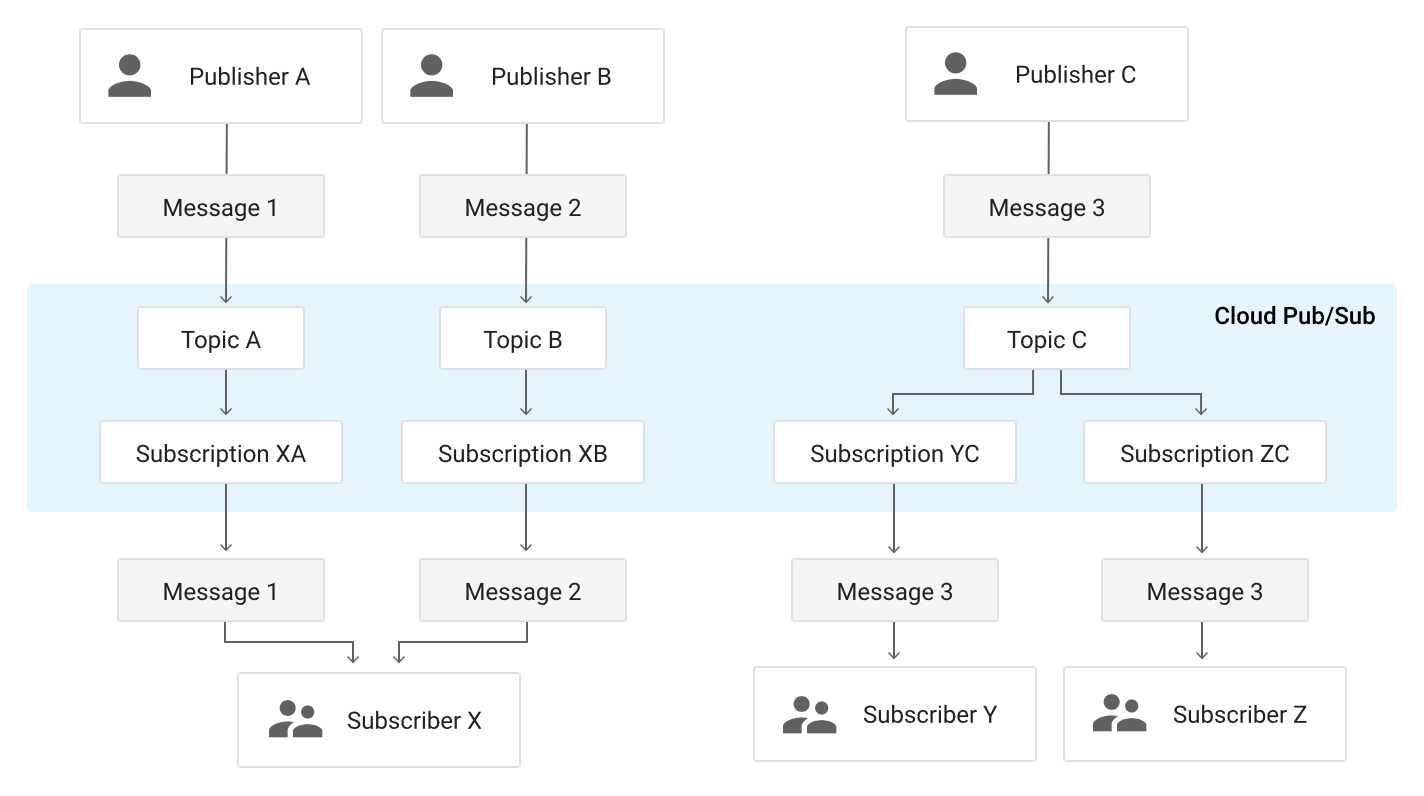
\includegraphics[width = 15.5cm]{figures/pubsub_img1}
    \caption{Example of a publisher-subscriber relationships}
    % \label{fig:prev}
\end{figure}

In this scenario, there are two publishers publishing messages on a single topic. There are two subscriptions to the topic. The first subscription has two subscribers, meaning messages will be load-balanced across them, with each subscriber receiving a subset of the messages. The second subscription has one subscriber that will receive all of the messages. The bold letters represent messages. Message A comes from Publisher 1 and is sent to Subscriber 2 via Subscription 1, and Subscriber 3 via Subscription 2. Message B comes from Publisher 2 and is sent to Subscriber 1 via Subscription 1 and to Subscriber 3 via Subscription 2.

\vspace{0.4cm}
\textbf{A practical example}
\vspace{0.4cm}

\begin{lstlisting}[language=Python, caption=Python example Pub/Sub]
# This function sends the weather measurements at a given rate. 
def weather_data_pubsub_comm():
    publisher = pubsub_v1.PublisherClient()
    topic_path = publisher.topic_path('savage2251', 'temp-1')
    try:
        t = threading.currentThread()
        while getattr(t, 'do_run', True):
            data = {'temperature': weather.temperature,
                    'air_pressure': weather.pressure,
                    'color': {
                        'red': colour.red, 
                        'green': colour.green, 
                        'blue': colour.blue, 
                        'clear': colour.clear
                    },
                    'light': amb_light.light,
                    'event_time': datetime.today().isoformat()
            }

            data = json.dumps(data)
            data = data.encode('utf-8')
            future = publisher.publish(topic_path, data=data)
            time.sleep(sleep_delay)
    except FlotillaException:
        print('Stopping Flotilla..'); 
        dock.stop()
\end{lstlisting}

\subsection{Cloud BigQuery}

BigQuery is a serverless, highly scalable, and cost-effective cloud data warehouse that has built-in machine learning capabilities. The main reason behind its usage in this project is to query streaming data in real time and get up-to-date information.

\vspace{0.4cm}
\textbf{BigQuery ML}
\vspace{0.4cm}

The BigQuery ML enables users to create and execute machine learning models in BigQuery using standard SQL queries. A model represents what an ML system has learned from the training data \cite{bigQuery}. The following types of models are supported by BigQuery ML:
\begin{itemize}
    \item{Linear regression for forecasting; for example, the sales of an item on a given day. Labels are real-valued (they cannot be +/- infinity or NaN).}
    \item{Binary logistic regression for classification; for example, determining whether a customer will make a purchase. Labels must only have two possible values.}
\end{itemize}

Other machines learning models that are accessible, though we did not use in this project are:
\begin{itemize}
    \item{Multiclass logistic regression for classification. These models can be used to predict multiple possible values such as whether an input is "low-value," "medium-value," or "high-value." Labels can have up to 50 unique values. In BigQuery ML, multiclass logistic regression training uses a multinomial classifier with a cross entropy loss function.}
    \item{K-means clustering for data segmentation; for example, identifying customer segments. K-means is an unsupervised learning technique, so model training does not require labels nor split data for training or evaluation.}
    \item{TensorFlow model importing. This feature allows you to create BigQuery ML models from previously-trained TensorFlow models, then perform prediction in BigQuery ML. See the CREATE MODEL statement for importing TensorFlow models for more information.}
\end{itemize}

\vspace{0.4cm}
\textbf{A practical example}
\vspace{0.4cm}

\begin{lstlisting}[language=SQL, caption=BigQuery ML query example]
-- This query was used to find an estimative distannce one can run given as input the starting hour of the event.
CREATE or REPLACE MODEL fitness.hourly_activities
OPTIONS
  (model_type='linear_reg', labels=['distance']) AS

WITH params AS ( 
        SELECT 0 AS TRAIN, 1 AS EVAL),
     activities AS (
        SELECT 
          distance,
          EXTRACT(HOUR FROM start_date) AS hourofday,
        FROM 
          `savage2251.bachelor.activities`, daynames, params
        WHERE
          moving_time > 0 and 
          distance > 0 and 
          MOD(ABS(FARM_FINGERPRINT(
            CAST(start_date AS STRING))), 2) = params.TRAIN
        ORDER BY hourofday)

SELECT * FROM activities
\end{lstlisting}

\section{Summation} 

At the end of this section the reader should have a better understanding of state of the art technologies involved in mining data streams, wearable sensors trends in fitness, and the implications of 3D printing in the process of rapid-prototyping. The products presented are mature, currently available, used in production by other companies and individuals, and well documented. These tools make data exploration possible from a software engineering standpoint, so in the following section we will approach strategies of finding knowledge through mathematicals models and numeric calculus.